
\documentclass[draft,linenumbers]{agujournal}
\draftfalse
\journalname{Journal of Advances in Modeling Earth Systems (JAMES)}
\begin{document}


\title{Implementing plant hydraulics in the Community Land Model}
\authors{Daniel Kennedy\affil{1},
Sean Swenson\affil{2},
Keith Oleson\affil{2},
David Lawrence\affil{2},
Rosie Fisher\affil{2},
Pierre Gentine\affil{1}
}


\affiliation{1}{Columbia}
\affiliation{2}{National Center for Atmospheric Research, Table Mesa Drive, Boulder, Colorado, USA}
\correspondingauthor{Daniel Kennedy}{djk2120@columbia.edu}

\begin{keypoints}
\item A simplified soil-plant-atmosphere continuum model based on hydraulic theory is implemented in the Community Land Model (version 5).
\item Prognostic leaf water potential replaces soil matric potential as the basis for stomatal conductance water stress. 
\item Prognostic root water potential is used to implement hydraulic root water uptake, replacing the heuristic soil 'wilting' factor .
\end{keypoints}



\begin{abstract}
= enter abstract here =
\end{abstract}

%====================
%  INTRODUCTION
%====================

\section{Introduction}

Trees face emerging climate change risk globally \citep{allen2010,anderegg2013b}.
Understanding vegetation response is a high priority, both for discerning climate impacts and for modeling feedbacks to the carbon and hydrological cycles.
In addition to stress from soil moisture drought, vegetation is susceptible to increasing atmospheric demand \citep{restaino2016,novick2016b,lemordant2018}.
Increases in vapor pressure deficit (VPD) have occurred with global warming \citep{ficklin2017,seager2015}, and are associated with impacts on vegetation (e.g., large-scale die-off) \citep{williams2013,mcdowell2015}.
Significant uncertainty remains regarding how vegetation will respond to changes in hydroclimate within Earth System Models, feeding back onto the carbon cycle as vegetation mediates carbon uptake \citep{dekauwe2017,friedlingstein2014,trugman2018}.


Plant water stress parameterizations are important in Earth System Models, as they define vegetation regulation of surface fluxes (photosynthesis, transpiration) to water fluctuations.
Vegetation water use strategies also modulate carbon uptake, creating a critical coupling between the Earth System's carbon and hydrological cycles \citep{green2017}.
Drought stress parameterizations (functions which relate simple metric of soil moisture status to leaf gas exchange) are widely used to define the response of stomatal conductance to vegetation water status that is used to attenuate transpiration, photosynthesis, and root water uptake with drying.
The dynamics of this water stress representation in models have broad effects on critical land surface processes \citep{joetzjer2014}, such as photosynthesis rates.
On daily and weekly time scales, Water stress parameterizations influence the partitioning of latent versus sensible heat, as it modified the Bowen ratio (Gentine et al., 2007, 2001). This in turn feeds back onto surface and air temperature, though land-atmosphere feedbacks \citep{bonan2014}.
On longer timescales vegetation water use strategies regulate the global carbon and water cycles \citep{dekauwe2015}.

Several recent studies have aimed at advancing the representation of water flow through the Soil-Plant-Atmosphere continuum (SPAC) in land-surface and ecosystem models \citep{xu2016,christoffersen2016,sperry2017}.
Explicit modeling of water flow through the SPAC adds complexity, but is consistent with evidence of dynamic regulation of vegetation water use in response to both soil and atmospheric drying \citep{sperry2015}.
Furthermore, becasue they are based on Darcy's Law, SPAC models have a robust physical basis compared to empirical water stress formulations.
SPAC models involve new parameters, which presents challenges \citep{drake2017}, but plant hydraulic trait information is available \citep{kattge2011,anderegg2015a}, providing constraints on parameter estimation.   and which can be informative of species vulnerability to drought \citep{choat2012}.
Likewise vegetation water status observations are now available from remote sensing platforms, at a scale that is directly comparable to model development \citep{konings2016,grant2016} and therefore can be used to validate model results \citep{momen2017,konings2017b}.

Specifically, the empirical representation of vegetation water stress in the Community Land Model (CLM) and other land surface models has been a known deficiency, with implications for the representation of the dry/wet season in tropical rainforests for example \citep{powell2013,ukkola2016}. Indeed, recent studies suggest that the soil water stress parameterization introduces model bias in turbulent fluxes \citep{bonan2014} and contributes to unrealistic drought response of photosynthesis and stomatal conductance \citep{powell2013}.

In this study, we develop a new plant water stress parameterization within the recently released CLM version 5 (CLM5), based on hydraulic theory, which we refer to as the 'Plant Hydraulic Stress' (PHS) configuration. 

Adding the representation of the SPAC introduces the representation of vegetation water potential (discretized into leaf, stem and root elements) into the CLM, as well as an explicit representation of water supply, from the soil through the vegetation substrate. Transpiration is attenuated in the model with drought stress according to leaf water status, capturing dynamic vegetation water use regulation. These changes in the parameterization framework have numerous implications, including 

1. Leaf water potential serves as a metric for water status compared to soil water or soil matric potential. As such, it reflects vegetation sensitivity to both soil and atmospheric drying, while serving as a diagnostic for excessive xylem tension and cavitation risk. 

2. Modeling plant hydrodynamics allows representing hydraulic redistribution \citep{lee2005}, as the flow respects Darcy's law and thus is always directed down gradients of water potentials. 

3. Further, root water potential can be used to predict gradient-based root water uptake based on Darcy's law, replacing the previous empirical transpiration partitioning heuristic. This provides the means to vary, for example, the mean depth of extraction with changing soil water conditions.

4. The new model can represent a range of water use strategies (i.e. isohydricity and anisohydricity), improving the connection between plant carbon allocation and water availability.

5. Modeling vegetation water potential allows improved connection to remote sensing observations of vegetation water status ( Vegetation Optical Depth) \citep{konings2016}. 

To assess the new model formulation, we carried out site-level simulations at Caxiuan\~a National Forest in Brazil, which features a critical biome (terra-firme moist tropical evergreen forest) \citep{fisher2006}.  Starting in 2001, a plot at this site was subjected to an approximately 50\% percent precipitation through-fall exclusion. Due to the large drop in soil moisture at the precipitation exclusion site, significant vegetation water stress regulation of transpiration and photosynthesis was present at the site, providing a natural experiment to test the model \citep{fisher2007}.

In this paper we therefore:
1. Introduce the PHS theory and implementation in the CLM
2. Analyze the dynamics of modeled water stress, root water uptake and soil moisture profiles. 
3. Compare PHS to the behavior of the previous CLM water stress configuration.
4. Discuss the benefits and limitations of the new model. 

SAY IN WHICH SECTION WE WILL FINE EACH PART

%====================
%  MODEL DESCRIPTION
%====================
\section{Model Description}

%Photosynthesis
\subsection{Photosynthesis}
\label{sect:A}
    The CLM5 photosynthesis model is described in details in \citet{bonan2011}, \citet{thornton2007},
    and \citet{oleson2013}. Photosynthesis is limited by three factors: Rubisco-limitations, light-limitations, and export-limitations 
    following \citet{farquhar1980} and \citet{harley1992}. The implementation extends \citet{sellers1996a,sellers1996b} with 
    co-limitation following \citet{collatz1991}. 
    
    The CLM5 photosynthesis module, in its default configuration, is a two-big-leaf model, with a sunlit and shaded leaf for each plant functional type \citep{thornton2007, dai2004, oleson2013}. 
    The canopy fluxes module iterates the solution for leaf temperatures to satisfy the leaf surface energy balances on both sunlit and shaded leaves, while environmental conditions are evolving.
    Within this, the photosynthesis module further iterates to solve for inter-cellular CO$_2$ concentration, balancing stomatal flux of 
    CO$_2$ with photosynthetic assimilation flux of CO$_2$.
    

%Stomatal Conductance
\subsection{Stomatal Conductance}
\label{sect:gs}
    CLM5 implements the Medlyn stomatal conductance model, which reconciles the empirical and optimal approaches to 
    stomatal conductance \citep{medlyn2011}.. 
    The optimization aims to maximize photosynthesis relative to transpiration costs. 
    Stomatal conductance of CO$_2$ is thus directly related to net photosynthesis ($A_n$) 
    and inversely related to the square root of the vapor pressure deficit near the leaf surface ($\sqrt{D}$) and the concentration of CO$_2$ at the leaf surface ($C_a$).
    \begin{equation}
    g_s=g_0+\left(1+\dfrac{g_1}{\sqrt{D}}\right)\dfrac{A}{C_a}
    \end{equation}
    The model features two parameters $g_0$ ($\mu$mol / m2 / s) and $g_1$ (kPa$^{0.5}$). 
    The $g_0$ parameter is minimum stomatal conductance, representing cuticular and epidermal losses (small). 
    The $g_1$ parameter relates to the marginal water cost guiding the optimization of carbon assimilation. 
    These parameters are plant functional type dependent.
    
    While maximizing assimilation relative to water transpiration costs ($A-\lambda E$), the Medlyn model does not 
    but does not resolve concurrent limitations to stomatal conductance associated with declining soil water. 
    To represent soil water stress, and its impact on leaf-gas exchange, land surface models typically include a `water stress factor' (see section zqz). 

    
\subsection{Water stress factor}

    In the CLM the water stress factor ($f_w$) multiplies the `well-watered rate' of maximum carboxylation ($V_{\text{cmax,ww}}$) to effect water stress (as described in \citet{oleson2013}). 
    
    \begin{equation}
    V_{\text{cmax}} = f_w\, V_{\text{cmax,ww}} 
    \end{equation}

    Other models opt for stomatal limitation based on soil moisture, linking the stomatal conductance model slope parameter to soil moisture (e.g. \cite{manzoni2011}, which modulates $\lambda$ based on soil water).
     However, \cite{lin2018} found that only the intercept parameter was sensitive to soil moisture based on eddy-covariance observations.
    \cite{zhou2013} suggest that changes in assimilation tend to exceed those predicted by modulating $g_1$ with soil moisture, but could be captured by changing $V_{\text{cmax}}$.
    Other field studies, however, suggest that measured $V_{\text{cmax}}$ at the leaf level does not change with drought \citep{flexas2004}. 
    On the other hand, the modeled $V_{\text{cmax}}$ is a bulk measure of $V_{\text{cmax}}$ and may implicitly account for mesophyll conductance changes \citep{rogers2017}, which has been shown to be water stress dependent \citep{flexas2012}.

    Uncertainty remains within the literature for how and where to apply water stress factors to photosynthesis and/or stomatal conductance 
    \citep{zhou2013,novick2016a,sperry2015}.
    For now, applying water stress through $V_{\text{cmax}}$ seems well-supported, but future refinements may well be appropriate.
    In this study, we preserve the location of water stress, but experiment with how $f_w$ responds to environmental conditions.
    
    \subsubsection{Soil Moisture Stress (control model)}
    
    The control model for our study is Soil Moisture Stress (SMS), which we compare to the model of interest, Plant Hydraulic Stress (PHS). 
    PHS is the default configuration of CLM5.
    SMS is a re-configuration of CLM5, substituting in the CLM4.5 representations of 
    (1) root water uptake (Section \ref{sect:rwu}) and (2) water stress (described here).
    Otherwise the models are identical.
    
    The scalar $f_w$ is calculated as the summation of the soil wilting factor across the $n$ soil layers, weighted by root fraction ($r_i$).
    The soil wilting factor ($w_i$) is a bounded linear function of soil matric potential ($\psi_{\text{soil},i}$).
    The function is defined by two parameters, the soil potential with stomates fully open ($\psi_o$) and fully closed ($\psi_o$).  

    \begin{linenomath*}
    \begin{equation}
     f_{w,\text{SMS}} = \sum_{i=1}^{n}{r_iw_i}
    \label{bt:1}
    \end{equation}
    \begin{equation} 
    \label{bt:2}
    w_i=0 \leq \dfrac{\psi_{\text{soil},i}-\psi_{c}}{\psi_{o}-\psi_{c}} \leq 1
    \end{equation}
    \end{linenomath*}
    
    \subsubsection{Plant Hydraulic Stress (new model)}
    
    PHS introduces a new formulation of $f_w$, which is based on leaf water potential ($\psi_{\text{leaf}}$) instead of soil potential (details are provided in Section zqz).
    The relationship is modeled with a weibull function, subject to two parameters: the water potential at 50\% loss of stomatal conductance ($\psi_{50}$) and a shape-fitting parameter ($c_k$).
    
    \begin{linenomath*}
    \begin{equation}
    f_{w,\text{PHS}} = 2^{-\left(\dfrac{\psi_{\text{leaf}}}{\psi_{50}}\right)^{c_k}}
    \end{equation}
    \end{linenomath*}
    
    Utilizing leaf water potential instead of soil water potential for drought stress, introduces a new paradigm to the model. 
    Leaf water potential is modulated by supply of sap to the leaves and by evaporative demand, as regulated by stomatal dynamics \citep{novick2016a}. 
    As a result, low soil water (bottom-up stress) induces stress due to limited water supply, but in addition, high atmospheric VPD can induce stress with the associated increases in the gradient in water potential across the plant xylem (top-down stress). 
    This latter mechanism was absent from the previous water stress function (dependent on soil water potential only), by construction.
    Given the importance of rising VPD, it appears critical to include such mechanistic dependence of water stress though.
    The new stress factor formulation reflects the concept of hydraulic safety, with vegetation avoiding excessive xylem tension associated with risk of cavitation.
    While the Medlyn stomatal conductance model does depend on VPD, this captures water `costs' and not xylem tension.
    Discussion of the water stress factor continues in Section \ref{sect:stress}.

\subsection{Root Water Uptake}
\label{sect:rwu}
    The CLM features a vertically discretized soil column with variable soil layer thicknesses.
    The number of soil layers ($n$) can vary, depending on the depth to bedrock.
    Soil water movement in each soil layer is governed by Richards' equation, with root water uptake ($q_i$) incorporated as a sink term.
    Summed over the soil column, root water uptake is required to equal transpiration ($T$).

    \begin{linenomath*}
    \begin{equation}
    T = \sum^n_i{q_i}
    \end{equation}
    \end{linenomath*} 

\subsubsection{SMS}
    
    In the SMS configuration, a heuristic function is used to determine $q_i$.
    Transpiration is partitioned among the soil layers layers based on the product of the root fraction and the wilting factor, which must be normalized by $f_w$. 
    Substituting for $w_i$ yields the SMS root water uptake equation as a function of the layer-$i$ soil potential ($\psi_{\text{soil},i}$).
    
    \begin{linenomath*}
    \begin{equation}
    \label{bt:4}
    q_i = \dfrac{r_i w_i}{f_w}T
    \end{equation}
    \end{linenomath*}
    
    \begin{linenomath*}
    \begin{equation}
    q_i =
    \begin{cases}
    \label{eq:btrwu}
    0    & \text{if } \psi_{\text{soil},i}<\psi_{c}  \\
    \\[1pt]
        \dfrac{T}{f_w} \dfrac{r_i}{\psi_{o}-\psi_{c}} \left(\psi_{\text{soil},i}-\psi_{c} \right)     & \text{if } \psi_{c} \le \psi_{\text{soil},i} \le \psi_{o} \\
    \\[1pt]
    \dfrac{T}{f_w} r_i    & \text{if } \psi_{c} \le \psi_{\text{soil},i} \le \psi_{o}
    \end{cases}
    \end{equation}
    \end{linenomath*}
    
    In the Darcy framework, water fluxes are the product of hydraulic conductance ($k_i$) and hydraulic gradient ($\Delta\psi$).
    Upon inspection of (\ref{eq:btrwu}), we can define hydraulic analogs resulting from the transpiration partitioning heuristic function, 
    allowing easy comparison to the PHS root water uptake implementation.
    
    \begin{linenomath*}
    \begin{equation} \begin{aligned}
    q_i &= -k_i\Delta\psi \\
    \Delta\psi &=  \psi_{c}-\psi_{\text{soil},i} \\
    k_i &= \dfrac{T}{f_w} \dfrac{r_i}{\psi_{o}-\psi_{c}} \\
    \mbox{constrained by:} \qquad
    \Delta\psi &=
    \begin{cases}
    0                          & \text{if } \psi_{\text{soil},i}<\psi_{c}  \\
    \psi_{c}-\psi_{o} & \text{if } \psi_{\text{soil},i}>\psi_{o}
    \label{kb}
    \end{cases}
    \end{aligned}\end{equation}
    \end{linenomath*}
    
    
    \subsubsection{PHS}
    
    PHS installs an alternative to the SMS heuristic approach, using a mechanistic representation of root water uptake, following Darcy's Law.
    Instead of using a constant parameter ($\psi_c$) for defining $\Delta\psi$, PHS installs a physical model of vegetation water potential (described in Section \ref{sect:vwp}).
    Fluxes from a given soil layer are driven by the gradient between soil potential ($\psi_{\text{soil},i}$) and the water potential in the root collar ($\psi_{\text{root}}$), 
    after accounting for the effects of gravity ($\rho g z$, where $z$ is the soil layer depth).
    Hydraulic conductance across the soil and roots ($k_{sr}$) is modeled based on soil hydraulic properties and xylem vulnerability, 
    accounting for the path across the soil matrix and through the xylem conduits (details in Appendix zqz).
    
    \begin{linenomath*}
    \begin{equation}
        \begin{aligned}
    q_i &= -k_{sr}  \left(\psi_{\text{root}}-\psi_{\text{soil},i}+\rho g z\right)
    \label{phs:sink}
    \end{aligned}
    \end{equation}
    \end{linenomath*}
    
% Plant Hydaulics
\subsection{Modeling Vegetation Water Potential}
\label{sect:vwp}
  The PHS model within CLM5 uses Darcy's law to model the flow of water through the SPAC, which can be represented with an electrical circuit analogy (Figure \ref{circuit}).
  PHS solves for vegetation water potential along the path from soil-to-atmosphere.
  Vegetation water supply (root water uptake) and demand (transpiration) are both coupled to water potential, and the solution for vegetation water potential is the set of values that matches supply with demand.

  \begin{figure}[h]
     \centering
     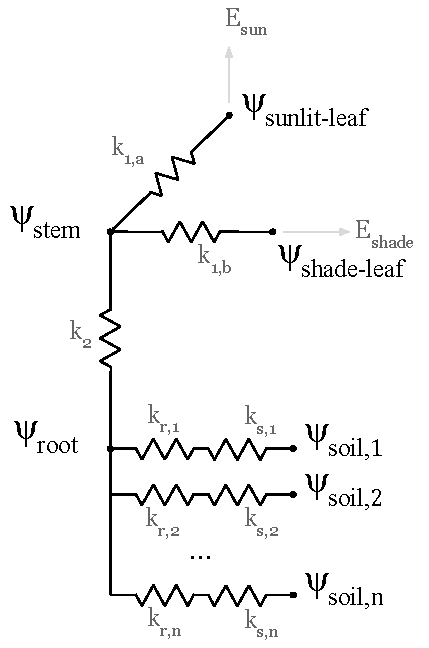
\includegraphics[width=9pc]{../figs/circuit.pdf}
     \caption{Plant hydraulic circuit analog schematic}
     \label{circuit}
  \end{figure}


  PHS solves for vegetation water potential at four locations: $\psi_{\text{root}}$, $\psi_{\text{stem}}$, $\psi_{\text{shade-leaf}}$, and $\psi_{\text{sun-leaf}}$.
  The number of nodes is chosen as the strict minimum to allow allow for differences in segment parameterizations \citep{simonin2015, sperry2015}, while also conforming to existing CLM model structure (vertical discretized soil layers, 2-big-leaf).
  At each node in the circuit diagram in Figure \ref{circuit} we model water potential, and, between nodes, we resolve the flux of water based on Darcy's law. 
  Water uptake from the different soil layers is assumed to operate in parallel; a typical assumption justified by higher resistance in lateral versus central roots (e.g. Williams et al. 2001). 
  Two resistors operate in series between each $\psi_{\text{soil}}$ and $\psi_{\text{root}}$, to represent the path across the soil matrix and then through the root tissue \citep{williams1996}. 
  Specifics on the parameterization of conductance for each segment are provided in Appendix B.1.

%Water Supply
    \subsubsection{Water supply}
    \label{sect:supply}
    Water supply is modeled via Darcy's Law, where flux of water ($q$) is the product of the path hydraulic conductance ($k$) and the gradient in water plus gravitational potential $psi$.  Equation \ref{eq:darcy} represents the flow from a generic node 1 to node 2. 
    
     \begin{linenomath*}
     \begin{equation}
     \label{eq:darcy}
     q = -k\left(\psi_2 - \psi_1 - \rho g \Delta z\right)
     \end{equation}
     \end{linenomath*}
    
    For simplicity, PHS does not represent plant tissue water storage (or capacitance, using the electrical circuit analogy).  
    Capacitance significantly complicates the water potential solution \citep{celia1990} and is challenging to parameterize \citep{bartlett2016}. 
    However, buffering of water stress provided by tissue water storage could potentially be important especially on sub-daily timescales \citep{meinzer2009,epila2017}, 
    whereby its inclusion may be warranted in future model generations.

     Hydraulic conductance through vegetation segments is modeled following empirical xylem vulnerability curves \citep{tyree1989}, where segments lose conductance with increasing xylem tension related to cavitation and embolism \citep{holbrook2001}.
      The vulnerability curves model loss of conductance relative to maximum conductance ($k_{\text{max}}$) using two parameters: 
      $c_k$, a sigmoidal shape-fitting parameter, and $p_{50}$, the water potential at 50\% loss of segment conductance (following \cite{gentine2016}). 
     
     Both $c_k$ and  $p_{50}$ can be estimated from field experiments \citep{sack2002}, and $p_{50}$ is available in the TRY trait database \citep{kattge2011}. 
     Parameterization based on $p_{50}$ aligns with the call for a transition to models that use a wider range of plant functional trait data in their parameterization \citep{anderegg2015a}. 
     The loss of xylem conductivity is based on lower terminal water potential ($\psi_1$) as is typical in other simplified models \citep{xu2016}, but 
     may underestimate the integrated loss of conductivity \citep{sperry2015}. 
         
     \begin{linenomath*}
     \begin{equation}
     \label{eq:vulnerability}
     k = k_{\text{max}} \, 2^{-\left(\dfrac{\psi_1}{p_{50}}\right)^{c_k}}
     \end{equation}
     \end{linenomath*}
     
     PHS models root, stem, and leaf tissue conductances according to equation \ref{eq:vulnerability}. 
     The parameterization of $k_{\text{max}}$ varies by hydraulic segment (see details in Appendix B1). 
     The conductance across the soil matrix to the root surface follows \citet{williams2001} and \citet{bonan2014}. 
     Bulk soil resistivity is based on \citet{clapp1978} as described in \citet{oleson2013}. 
     Details are provided in Appendix B1.
    
%Water demand
    \subsubsection{Water demand}
    \label{sect:demand}
    
\citep{klein2014}, and multiplies $V_{\text{cmax}}$, attenuating photosynthesis, and thus also stomatal conductance and transpiration.

     \begin{linenomath*}
     \begin{equation}
     \begin{aligned}
     f_{w,sun} &= 2^{-\left(\dfrac{\psi_{\text{sun-leaf}}}{\psi_{50}}\right)^{c_k}} \\
     f_{w,shade} &= 2^{-\left(\dfrac{\psi_{\text{shade-leaf}}}{\psi_{50}}\right)^{c_k}} \\
     E_{sun} & = f_wE_{sun,max} \\
     E_{shade} & = f_wE_{shade,max}
     \end{aligned}     
     \end{equation}
     \end{linenomath*}
%PHS solution
    \subsubsection{PHS solution}
    \label{sect:solution}
    
    PHS solves for the set of vegetation water potential values ($\psi$) that matches water supply (root water uptake) to water demand (transpiration), while satisfying continuity across the four water flow segments (soil-to-root, root-to-stem, stem-to-leaf, and leaves-to-transpiration). 
    Beginning from an initial condition of $\psi$ (from the previous timestep), PHS computes the flux divergence $f$ (representing the mismatch of flow in and out of each segment) and iteratively updates $\psi$ until $f\to0$.
    
    \begin{linenomath*}
    \begin{equation} 
    \psi = \left[
    \begin{array}{c}
    \psi_{\text{sun}} \\ 
    \psi_{\text{shade}} \\ 
    \psi_{\text{stem}} \\ 
    \psi_{\text{root}}            
    \end{array} \right]
    \end{equation}
    \end{linenomath*}
    
    \begin{linenomath*}
    \begin{equation}
    f\left(\psi\right) = \left[ 
    \begin{array}{c}
    E_{sun}-q_{sun}\\
    E_{shade}-q_{shade}\\
    q_{sun}+q_{shade}-q_{stem}\\
    q_{stem}-\sum_{j=1}^n{q_{root,j}}
    \end{array} \right]
    \end{equation}
    \end{linenomath*}
    
    \begin{linenomath*}
    \begin{equation}
    A = \dfrac{df}{d\psi}
    \end{equation}
    \end{linenomath*}    
    
    While $\left|f\right|>0$
    \begin{linenomath*}
    \begin{equation} \begin{aligned}
    \label{eq:iter}
    \Delta\psi &=A^{-1}f\left(\psi_i\right) \\
    \psi_{i+1}  &= \psi_i + \Delta\psi
    \end{aligned} \end{equation}
    \end{linenomath*}    
    
    The numerics are tractable because $f$ has analytical derivatives and $A$ (a 4x4 matrix with six null entries) is easy to invert when well-conditioned. Supply and demand converge, because transpiration demand decreases with more negative leaf water potentials and supply increases with more negative leaf water potentials. Within a set of PHS iterations (\ref{eq:iter}), transpiration is assumed to be linear with $f_w$.
    
    The PHS loop is nested within iterations for intercellular CO$_2$ concentration and leaf temperature. The non-linear relationship between $f_w$ and transpiration is resolved through iteration for converging $f_w$ alongside intercellular CO$_2$. Details on the numerical implementation are provided in Appendix Section B.1.
   
%====================
%  EXP DESCRIPTION
%====================
\section{Experiment Description}
All four simulations in this paper use the same development version of CLM5 (development version r270, https://github.com/ESCOMP/ctsm/releases/tag/clm4\textunderscore 5\textunderscore 18\textunderscore r270).
The four simulations are used to assess the impact of the plant hydrodynamics model (PHS vs. SMS) on a through-fall experiment (i.e., with either ambient or 60\% through-fall excluded), with all other model components and forcing shared. Simulations are run offline (uncoupled from an active atmospheric model), spanning from 2001 through 2003, utilizing the satellite phenology (SP) mode of CLM5 in which vegetation state (LAI, canopy height) is prescribed and biogeochemistry is inactive. All simulations start from the same initial conditions, which are obtained from a 9-year spin-up that repeats the PHS/Ambient simulation three times. Descriptions of site characteristics, forcing data, and observational sap flux, can be found in \cite{fisher2007}.

\subsection{Parameter Values and Through-fall Exclusion}
\label{sect:param}
\begin{table}
\caption{Select parameter values}
\centering
\begin{tabular}{c c c c}
CLM name & Full Name & Symbol &  Value \\
\hline
kmax(1) & Maximum Sun Branch Conductance & $k_{1a,\text{max}}$ &  4e-8 s$^{-1}$ \\
kmax(2) & Maximum Shade Branch Conductance & $k_{1b,\text{max}}$ &  4e-8 s$^{-1}$ \\
kmax(3) & Maximum Stem Conductivity & $k_{2,\text{max}}$ &  4e-8 m/s \\
krmax & Maximum Root Conductivity & $k_{r,\text{max}}$ &  6e-9 m/s \\
psi50 & Water potential at 50\% loss of conductivity & $\psi_{50}$ &  -1.75 MPa \\
ck & Vulnerability shape parameter & $c_k$ &  2.95 \\
smpso & Soil potential with stomata fully open & $\psi_o$ & -0.65 MPa \\
smpsc & Soil potential with stomata fully closed & $\psi_c$ & -2.5 MPa \\
medlyn\textunderscore intercept & Medlyn intercept & $g_0$ &  100 $\mu$mol / m2 / s \\
medlyn\textunderscore slope & Medlyn slope & $g_1$ &  6 kPa$^{0.5}$ \\
n & Soil porosity to 4.64 meters & $n$ & 0.42 \\
n & Soil porosity beyond 4.64 meters & $n$ & 0.28 \\
hksat & Saturated soil hydraulic conductivity & $k_{\text{s,max}}$ & 3e-5 m/s \\
sucsat & Saturated soil matric potential & $\psi_{\text{sat}}$ & 461 Pa \\
bsw & Brooks-Corey parameter & $b$ & 6 \\
\hline
\end{tabular}
\end{table}

Selected parameter values concerning vegetation hydrodynamics are presented in Table 1. All other parameters use the default values associated with the r270 version of CLM5. Informed by \cite{fisher2008}, we tuned soil hydraulic parameters and through-fall exclusion rates to reasonably capture the observed soil water dynamics (\cite{fisher2007} Figure 4), Supplementary Figure \ref{top3m}. Likewise, we tuned $k_{max}$ and $g_1$ parameters to improve the fit to sap flux observations in the ambient simulation. The primary objective here is to present the dynamical impact of PHS tin terms of model functionality, rather than model performance, hence the choice to minimize model tuning. 

  \begin{figure}[h]
     \centering
     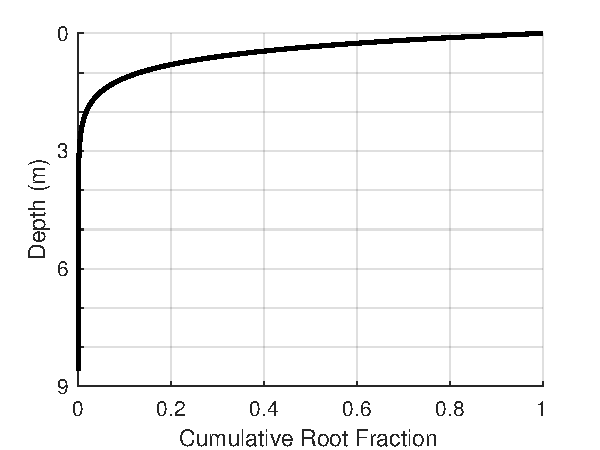
\includegraphics[width=20pc]{../figs3/roots.pdf}
     \caption{Cumulative rooting distribution}
     \label{roots}
  \end{figure}

%====================
%  RESULTS
%====================
\section{Results}  
\subsection{Vegetation water potential}

    
    Under ambient conditions, 2003 dry season (September-October-November) model average sunlit leaf water potential is -1.65 MPa at midday (local time 12-14h, Figure \ref{fig:vwp}a). 
    The midday pressure drop is primarily between $\psi_{root}$ and $\psi_{stem}$, representing the root collar and upper stem, respectively.
    Under TFE, model midday leaf water potential decreases to -2.31 MPa (Figure \ref{fig:vwp}b). 
    Partitioned among the segments of the SPAC, the changes in leaf water potential (totaling -0.66MPa) due to TFE are:
    -0.44MPa soil potential,
    -0.66MPa soil-to-root,
    +0.45MPa root-to-stem, and 
    -0.001MPa stem-to-leaf.
    This comports with previous evidence that seasonal changes in hydraulic resistance are larger belowground \citep{fisher2006}.
    
    Modeled root water potential values match wet season observations, but are less negative than dry season observations under ambient conditions \citep{fisher2006}.
    Midday leaf water potential features a seasonal cycle, with lower values during the dry season (Figure \ref{fig:vwp}c).
    Modeled leaf water potential values under ambient conditions are less negative than averages reported by \cite{fisher2006} (1.71 MPa during the wet season and -2.47 MPa during the dry season), but are within the range of observations.
    The model seems to underestimate isohydricity (i.e. minimal leaf water potential drop during drought) in response to TFE, showing a drop in leaf water potential of 0.66MPa (dry season, 2003), whereas observations showed no significant difference \citep{fisher2006} . Tweaking of the stomatal parameter could resolve such discrepancy. 


\subsection{Stress factor}
    
    Average midday stress values are comparable during the 2003 dry season (Figure \ref{fig:stress1}) with the two model configurations.
    Under ambient conditions, the average stress factor values are 0.59 and 0.54 for SMS and PHS, respectively (dry season, midday), 
    decreasing to 0.16 and 0.21, with TFE.
    While the SMS stress factor has minimal diurnal variability (Figure \ref{fig:stress1}a),
    PHS features increased stress at midday (Figure \ref{fig:stress1}b), corresponding to the drop in leaf water potential (Figure \ref{fig:vwp}b,c).
    Indeed, the PHS stress factor responds to both soil moisture and VPD (Figure \ref{fig:stress2}c,d), while SMS responds only to soil moisture (Figure \ref{fig:stress2}a,b).
    This dependence on VPD results in more wet season (FMA) stress with PHS (as compared to SMS) under both ambient and TFE conditions (Figure \ref{fig:gpp}a-d).

\begin{table}
\caption{Root-zone soil potential $^a$ (MPa) terciles for Figure \ref{fig:stress2}}
\label{tab:tercile}
\centering
\begin{tabular}{c c c }
Simulation & T1 & T2 \\
\hline
SMS, Ambient & -0.01 & -0.54 \\
SMS, TFE & -0.29 & -1.74 \\
PHS, Ambient & -0.01 & -0.05 \\
PHS, TFE & -0.05 & -0.33 \\
\hline
\multicolumn{2}{p{.5\linewidth}}{$^{a}$SMS values correspond to daily mean root-fraction weighted soil potential.
PHS values correspond to predawn root water potential.}
\end{tabular}
\end{table}


\subsection{GPP and Transpiration}
    The two models predict similar total GPP across 2002-2003 under TFE, with 3.96 kg/m$^2$ for SMS and 4.00 kg/m$^2$ for PHS, 
    but GPP is lower for PHS under ambient conditions (4.86 kg/m$^2$) as compared to SMS (5.46 kg/m$^2$, Figure \ref{fig:gpp}e-h).
    Seasonal variability in GPP is smaller with PHS. 
    The standard deviations of daily GPP (2002-2003) are 0.49 and 1.55 g/m2/d for AMB/TFE, 
    as compared to 1.53, 2.73 g/m2/d with SMS. 
    Transpiration seasonality is present in both models (Figure \ref{fig:t}a,b), but with a larger amplitude for SMS.
    PHS yields a better fit to field observations of daily sap flux (see Section zqz), with higher R$^2$ and lower RMSE compared to SMS 
    under both ambient and TFE conditions (Figure \ref{fig:t}c-f).

    
\subsection{Root water uptake: dynamics}
    Root water uptake is more sensitive to soil potential with PHS (Figure \ref{fig:rwu}),
    which follows from sharp declines in hydraulic conductance with drying.
    Hydraulic conductance decreases approximately by three orders of magnitude across the range of PHS soil potential (Supp Figure \ref{supp:cond}b).
    The SMS-implied conductance increases with more negative soil potentials, until $\psi_{\text{soil}}$ reaches -2.5MPa, beyond which it is defined to equal 0 (Supp Figure \ref{supp:cond}a).
    Root water uptake still decreases with SMS as soils dry, but only because of the decrease in $\Delta\psi$ (Supp Figure \ref{supp:cond2}c).
    Whereas PHS imparts a diurnal cycle to root water uptake through dynamic root water potential, 
    the hydraulic gradient with SMS is defined by $\psi_c$, which is constant, requiring a diurnal cycle in the implied conductance (Supp Figure \ref{supp:cond2}).
    
\subsection{Root water uptake: profiles}
    Overall, the two model configurations feature comparable transpiration during the dry season under ambient conditions (PHS: 28.3cm, SMS: 28.5cm).
    However they feature distinct vertical profiles, where PHS removes less water from intermediate soil layers (0.5-1.5meters) (Figure \ref{fig:qdry}d).
    SMS removes more water from these layers, due to the lower sensitivity of root water uptake to soil potential.
    Likewise partitioning of root water uptake within the soil column is more sensitive to precipitation in PHS (Figure \ref{fig:qdry}a-c). In PHS, during the longer periods without rain, surface extraction plateaus and transpiration is fueled by the deeper soil water.
    After rain events, surface extraction renews, while at depth, root water fluxes reverse, with water deposited instead of being extracted.
    Both models decrease surface extraction under TFE (Figure \ref{fig:qdry}b), but PHS has a larger compensation from beyond 2m (Figure \ref{fig:qdry}c),
    allowing more overall transpiration (14.6 vs. 10.8 cm).
    
    During the wet season PHS utilizes more water from the near-surface soil layers (Figure \ref{fig:qwet}b), 
    with zero net root water uptake beyond 35.2 cm in ambient conditions (or beyond 9.6cm under TFE).
    SMS extracts 49.8\% (AMB) and 81.5\% (TFE) of total transpiration from beyond those levels (Figure \ref{fig:qwet}). 
    PHS does extract farther into the soil profile, but in service of hydraulic redistribution, 
    sending the water deeper into the soil column.
        
\subsection{Hydraulic redistribution}
    SMS precludes hydraulic redistribution (HR) contrary to PHS, setting root water uptake to zero when reversed gradients in water potential occur.
    With PHS, in our experiment,  HR totals to 38.9 cm under ambient conditions in 2003 and 40.0 cm under TFE, with the majority (28.0, 26.7 cm) of this HR occurring at night (Figure \ref{fig:hr}).
    HR occurs in both directions (Supp Fig \ref{supp:hr}), but is predominately downwards (amb: 30.7cm, tfe: 33.8cm).
    Likewise HR occurs during both the wet and dry seasons.
    The seasonality changes with TFE, as AMB has more HR during Sept-Jan, while TFE features more HR during Feb-Apr.

\subsection{Soil moisture}
    During the dry season, SMS simulations yield much lower values for soil matric potential (Figure \ref{fig:sm}, Supp Fig \ref{supp:sm}). 
    During SON, SMS average soil potential is -1.42 MPa under ambient conditions. 
    Predawn root water potential averages to -0.14 MPa during SON-2003 under ambient conditions.
    With TFE, SMS dry season soil potential drops to -2.51 MPa and PHS to -0.50 MPa.

    PHS better matches observations of soil moisture, with RMSE lower by up to 55\% (Figure \ref{fig:sm2}, Supp Fig \ref{supp:sm2}).
    The SMS values correspond to a significant dry bias (Figure \ref{fig:sm2}), especially in the first meter of the soil column.
    This is associated with the soil wilting parameter ($\psi_c$), which takes the value -2.5MPa for the broadleaf evergreen tropical PFT \citep{oleson2013}.
    Note that this value is equivalent to the SMS average under TFE in the last paragraph.
 
\subsection{Soil moisture effect on transpiration}    
    Model soil potential shows limited relationship to sap flux observations under ambient conditions (Supp Fig \ref{supp:cool}b,f).
    However, in the SMS configuration, modeled transpiration decreases strongly with more negative soil potential (Supp Fig \ref{supp:cool}a),
    biasing the model relative to observations (Fig \ref{fig:cool}a).
    
    Sap flux observations under TFE show a stronger relationship with soil potential especially with PHS (Supp Fig \ref{supp:cool}h,d).
    With SMS, the modeled attenuation of transpiration with soil potential again seems to bias modeled transpiration with SMS (Fig \ref{fig:cool}b).
    Derived from $\psi_c$, transpiration approaches zero when soil potential reaches -2.5 MPa (Supp Fig \ref{supp:cool}c).
    The two PHS simulations feature less structure in transpiration bias vs. soil potential and less bias overall (Fig \ref{fig:cool}c,d).
    
\section{Discussion}
\subsection{The promise of plant hydraulics}
    Plant hydraulics can potentially improve model predictions of vegetation response to climate change \citep{sperry2015}, 
    especially if parameter ranges and model complexity can be constrained \citep{rogers2017}.
    Numerous site-level models have deployed plant hydraulics (e.g. \citet{williams1996,sperry1998,bohrer2005}), and studies show
    vegetation water potential can improve predictions of stomatal response to the environment \citep{sperry2017,anderegg2017},
    More recently hydraulics have been coupled to global models \citep{bonan2014,xu2016,christoffersen2016}, 
    but most Earth System Models do not provide a mechanistic representation of vegetation water dynamics.

    In this study, we have implemented plant hydraulic theory within CLM5, 
    using dynamic vegetation water potential to modulate leaf gas exchange and root water uptake.
    We model water potential according to a simplified circuit analogy (Figure \ref{circuit}), 
    which captures expected diurnal and seasonal dynamics of soil and vegetation water potentials, with lower values at midday within the stem and during the dry season (Figure \ref{fig:vwp}).
    Our model places the bulk of hydraulic resistance aboveground (Figure \ref{fig:vwp}a), 
    while the added resistance from dryness (TFE) is primarily loacted within the soil-to-root interface (Figure \ref{fig:vwp}b), consistent with previous results \citep{fisher2006}.
   

    Support for hydraulic models include improvements in modeling mortality and productivity \citep{mcdowell2018,choat2012}.
    However, concerns exist in the literature regarding hydraulic model complexity and parameterization \citep{verhoef2014,drake2017}, 
    which led to a series of simplifications implemented in our model design (see Section zqz).
    Recent work suggests model complexity can be managed, given the significant coordination of hydraulic traits \citep{bartlett2016,christoffersen2016}.
    Furthermore incorporating plant hydraulics provides access to new streams of observational data for model validation.
    Vegetation water potential can be monitored in the field \citep{boyer1967} and has been shown to correlate with microwave remote sensing products \citep{momen2017}.
    Parameter values can be measured in the field \citep{sack2002} and are available in the TRY database \citep{kattge2011}.

\subsection{Water stress and stomatal conductance}
    \label{sect:stress}

    PHS models (sunlit and shaded) leaf water potential, which serves as the input to the water stress factor, 
    replacing the previous version based on soil water potential in SMS.
    This imparts a diurnal cycle to the water stress factor (Figure \ref{fig:stress1}), following the midday drop in leaf water potential induced by leaf-level VPD transpiration demand.
    As such, stress now depends on transpiration demand, and, in turn, leaf-level VPD and radiation (Figures \ref{fig:stress2},\ref{supp:fsds}).
    This is in addition to the VPD response of stomatal conductance, which is now based on the Medlyn model and features stomatal conductance proportional to VPD$^-0.5$, which serves to optimize carbon gain versus water losses \citep{medlyn2011}.
    Here we tried to implement a stomtal water stress functoin  that includes xylem tension stress, where vegetation must limit transpiration to avoid cavitation and embolism. Support for this exists in the literature \citep{novick2016a,sperry2017}, but there is still no consensus on the best functional form to be used \citep{zhou2013}. 
    
    The water stress factor exhibits a seasonal cycle, with lower values (indicating more stress) during the dry season.  
    However, the seasonal variation in water stress is smaller than with the control model (Figure \ref{fig:gpp}a-d).
    As a result PHS features less seasonal variability in GPP, especially under ambient conditions (Figure \ref{fig:gpp}e-h).
    The xylem tension constraint in PHS induces a negative feedback on GPP.
    Indeed, factors increasing GPP (e.g. more light) also increase xylem tension and stress, which opposes increases in GPP.
    \cite{restrepo2017} show that GPP increases at Caxiuana during the dry season, suggesting that PHS may improve the GPP seasonal cycle relative to the control model.
    
    PHS underestimates the seasonal cycle in transpiration under ambient predictions, and exhibits less seasonal variability than sap flux observations (Figure \ref{fig:t}a,c).
    We produce in both models a high bias in transpiration under TFE, similar to previous evidence showing that models tend to underestimate the effect of TFE \citep{powell2013}.
    Considerable uncertainty remains regarding the appropriate functional form of water stress.
    Further work could examine other permutations of water stress, and/or concurrent improvement in photosynthesis parameters and model structure.
    But already, PHS does improve transpiration predictions, 
    with lower RMSE and higher correlation compared to the control model, albeit with model tuning (Figure \ref{fig:t}).

\subsection{The extensive influence of $\psi_c$}
    Water stress in the SMS model configuration is largely determined by 
    $\psi_c$, the soil potential at which stomates are fully closed.
    For the Broadleaf Evergreen Tropical PFT, $\psi_c$ equals -2.5 MPa \citep{oleson2013}.
    Root water uptake scales with hydraulic gradient ($\Delta\psi$), and
    $\psi_c$ serves as the sink potential for soil water extraction ($\Delta\psi = \psi_{\text{soil}}-\psi_c$).
    This defines the slope with which root water uptake decreases with soil drying (Figure \ref{fig:rwu})
    and results in transpiration overall trending towards zero as column-average soil potential approaches -2.5 MPa (Supp Fig \ref{supp:cool}).
    
    Root water uptake from a given soil layer is defined to be zero whenever soil potential is more negative than $\psi_c$ (Figure \ref{fig:rwu}),  
    following from the definition of the SMS water stress factor (Section zqz).
    This sharp non-linearity tends to make soil potential decrease to and then hold at values equal to $\psi_c$ (Figure \ref{fig:sm}).
    As such, $\psi_c$ has strong influence on model output for both transpiration and soil moisture, despite limited empirical or physical basis \citep{rogers2017}.
    
\subsection{Structural improvements in modeling root water uptake}

    Using $\psi_c$ is required with SMS, because water potential is not resolved through the vegetation substrate.
    Instead of a constant parameter, PHS uses dynamic root water potential ($\psi_{\text{root}}$) as the sink for measuring the hydraulic gradient for root water uptake (Figure \ref{fig:vwp}).
    This provides a critical structural improvement for modeling root water uptake, consistent with extensive evidence of dynamic vegetation water potential (e.g. \cite{fisher2006}).
    PHS also eschews the constraints on $\Delta\psi$ imposed by SMS (see section zqz).
    
    Root water uptake is equal to the product of $\Delta\psi$ and hydraulic conductance $k$. 
    The conductance varies by soil layer and, with PHS, features mechanistic reductions based on root xylem vulnerability and soil hydraulic properties, 
    as is appropriate for hydraulic-based models \citep{cai2014,warren2014}.
    As a result the soil-root conductance features a strong, positive relationship with soil potential, decreasing by almost three orders of magnitude as the soil dries (Supp Fig \ref{supp:cond}).
    PHS $k_{sr}$ appropriately penalizes extraction from depth, due to decreasing root density and increasing xylem length, 
    whereby PHS favors surface extraction when water is available (Figure \ref{fig:qwet}).
    The model can overcome these penalties, with compensatory root water uptake observed with increased extraction from beyond 2 meters depth during the TFE dry season (Figure \ref{fig:qdry}).
    Dynamic root water potential (in tandem with declining $k$) gives the system more play, allowing the model to switch to the lower layers as the surface dries out.
    PHS allows $\Delta\psi$ to change sign, yielding a representation of hydraulic redistribution, which has been observed in Amazonian forests \citep{oliveira2005}.
    
\subsection{Hydraulic Redistribution (HR)}
    During 2003, modeled HR totals to 38.9 cm under ambient conditions and 40.0 cm with TFE (Figure \ref{fig:hr}) in PHS.
    In our simulations, as observed in the field \citep{burgess1998}, HR occurs in both directions vertically (Supp Fig \ref{supp:hr}).
    Modeled HR is mostly downwards, sending water shallower water from rain events deeper into the soil column and thus saving it for when it is most needed, i.e. dry season.
    This would seem to convey an advantage to deep-rooted individuals, banking water for later use out of reach of shallow-rooted competitors.
    HR can offer significant water subsidies during dry periods \citep{jackson2000} and has been highlighted as an important missing feature in CLM \citep{lee2005}.
    
    Some of the challenges we faced were that HR seemed to oversupply the top layer of the soil column (spanning 0 to 2 cm below ground) and thus significantly degraded modeled soil evaporation (not shown). 
    In lieu of this, we set the hydraulic conductance to zero in that uppermost layer, disallowing any root water uptake there.
    Furthermore, observations of HR are extremely difficult, and the degree to which HR actually occurs is unclear. 
    Unequivocal detection of HR involves the observation of reverse flow along transport roots, typically at rates close to the detection threshold of sap flow monitoring systems. 
    In our simulations, HR increases root water uptake by up to 52\% relative to transpiration alone (2003, TFE). 
    
    HR follows directly from Darcy's Law, occurring when water potential in a given soil layer is more negative than $\psi_{\text{root}}$,
    but it remains to be seen whether HR as modeled in this implementation is a feature or a liability.
    PHS may overestimate HR, given the simplified root system architecture \citep{bouda2017} 
    and the lack of an explicit representation of fine-root cavitation \citep{kotowska2015}.
    Other models, similar to the SMS paradigm, disallow HR by constraining root water uptake to be positive \citep{xu2016}.
    We view this first implementation of HR into the default versions of the CLM as a `null' hypothesis for the functioning of this process, and as a platform to allow further refinement from the plant hydraulics community. Isotopologues of water could be used as a tool to further constraint this redistribution in CLM in the future. 

\subsection{Soil moisture and its influence on transpiration}

    Partly due to HR, vertical and temporal gradients in soil potential are significantly reduced in PHS (Figure \ref{fig:sm}).
    This is also related to the root water extraction gradient, which is significantly smaller in PHS (Supp Fig \ref{supp:cond2}).
    The SMS sink potential ($\psi_c$, -2.5MPa), is significantly lower than PHS ($\psi_{\text{root}}$, Figure \ref{fig:vwp}).
    This is associated with a significant dry bias relative to observations in the SMS simulations, especially in the first meter of the soil column.
    PHS reduces soil moisture RMSE by up to 55\% relative to SMS (Figure \ref{fig:sm}).
    
    The relationship with soil water potential seems to bias SMS predictions of transpiration relative to sap flux observations (Figure \ref{fig:cool}a,b).
    Under ambient conditions, soil water shows little relationship with sap flux observations with either model configuration (Figure \ref{supp:cool}b,f), 
    but SMS modeled transpiration decreases strongly in response to soil drying.
    This is in line with \cite{bonan2014}, where the water stress factor was found to impose too much attenuation of transpiration.
    PHS features less structure in the relationship between transpiration bias and soil potential and less bias overall (Figure \ref{fig:cool}c,d).
    Likewise PHS yields a stronger relationship than SMS between soil potential and sap flux observations during TFE (Figure \ref{supp:cool}b,f).
    This represents a major development, given repeated calls to improve vegetation water stress in the next generation of terrestrial biosphere models \citep{powell2013,rogers2017}.
     

\subsection{Inconsistencies in SMS}
    
    \subsubsection{Constant pulling potential}
    With SMS, the water potential gradient is implicitly defined for each soil layer as the difference between the soil water potential in that layer ($\psi_i$) and a constant parameter, the soil water potential when stomata are fully closed ($\psi_{c}$). This parameter serves as the vegetation ``pulling'' potential for calculating the soil transpiration sink.
    
    Using a constant wilting point is inconsistent with extensive evidence from the field of dynamic vegetation water potential, and cohesion tension theory (CITATIONS NEEDED) driving the transpiration flow. Likewise the values for $\psi_{c}$ are quite negative, (-2.5 MPa for broadleaf evergreen tropical, BET, forests). \cite{fisher2006} measured midday stem potential consistently higher than -0.5 MPa during the wet season, and on average -1.69 and -1.53 MPa during the dry season in the control and exclusion plots, respectively.
    
    \subsubsection{Conductance dynamics}
    In SMS, in lieu of dynamic vegetation water potential, intra-day SMS soil sink dynamics derive from a highly variable conductance (CLARIFY). As inferred in Equation \ref{kb}, SMS conductance is modeled as a function of $T_{max}$, and three constant parameters. $T_{max}$ is highly dynamic, responding to the diurnal course in transpiration demand. This is inconsistent with general principles of porous media flow, where conductivity is a function of the hydraulic architecture and its wetted status.    Likewise, this representation of conductance does not represent the characteristic phenomenon where vessels lose conductance with drying.
      
    \subsubsection{No dependence on belowground carbon allocation}
    As is typical in water stress parameterizations, the SMS conductance is scaled by layer using an area basis, here using the relative vertical root fraction is used. With PHS, an absolute measure of root biomass is used (see Appendix Equation \ref{eq:rai}), so that the belowground water cycle interacts with carbon allocation to the roots. An absolute measure better conforms with the physics of porous media flow and better responds to varying carbon allocation strategies. For example, with SMS, if root mass doubles in every soil layer, the root access to water remains unchanged.

    \subsubsection{Lacks penalties for extraction from depth}
    Both PHS and SMS account for the effect of decreasing root area with depth (PHS, root area; SMS, root fraction), but PHS implements two other penalties for extracting water from deep in the soil column that are missing from SMS. The first is minor, but water extracted from depth must overcome gravity, amounting to about 0.01 MPa per meter in depth. This is missing from SMS and included with PHS.  Likewise, SMS ignores the fact that hydraulic conductance is generally taken to scale with the inverse of conducting length. Deeper roots feature longer root tissue conducting length, and root spacing within the soil is less dense, requiring longer conducting distances across the soil matrix.In PHS, both these processes result in diminished hydraulic conductance (UNCLEAR).

    \subsubsection{Constraints}
    With SMS, the gradient in water potential is constrained between 0 and the range of soil potential between parameters for stomata fully open and closed (Equation \ref{kb}). The upper constraint caps the gradient in water potential when soil potential reaches the value for stomata fully open ($\psi_o$=-0.65 MPa for BET). Darcy's Law predicts that the gradient in water potential would continue to increase until saturation matric potential. The lower constraint caps the gradient in water potential at zero, disallowing negative gradients. However, reversed water fluxes, caused by positive gradients in water potential from root to soil, have been observed in the field \citep{burgess1998}. Both constraints are eschewed with PHS.     

\section{Conclusion}

\subsection{Caveats}

    Modeling stomatal conductance and photosynthesis, especially subject to water stress, is an area of ongoing research. We use the Medlyn VPD-dependence model coupled to a hydraulic stress function that attenuates $V_{\text{cmax}}$. This complies with observations \citep{lin2018,zhou2013} that stress applied through $g_1$ underestimates attenuation of photosynthesis. However, there is no direct evidence of declines in $V_{\text{cmax}}$ at the leaf level with drought \citep{flexas2006}, whereby future work may seek to represent mesophyll conductance in CLM to correct such discrepancy.
    
    The model hydraulic supply representation is simplified, to reduce the model parameter and computational burdens.
    No capacitance.
    No integration of xylem or soil conductances vulnerability, instead based on lower node.
    No hysteresis in loss of conductance, xylem instantly regain conductance upon re-wetting.
    Leaf conductance simplified.
    Soil layers fully parallel, soil potential constant each time step.
    
    Parameter uncertainty is significant.
    Notions of hydraulic architecture will never perfectly fit on this modeling scale, especially in a PFT paradigm.
    Field measurements of hydraulic traits will help constrain parameter ranges, but mostly only aboveground.
    Flux observations can help to tune stress parameters.
    Parameter estimation for root functioning is significantly more challenging, given the difficulty in underground trait observations.
    Likewise observational constraints of vertically-resolved states and fluxes underground are scarce.
    Follow-up work will be geared towards parameter estimation and assessing model skill.

\subsection{Utility of modeling vegetation water potential}


    The PHS configuration of the CLM5 is, to our knowledge, the first Earth System Model with a representation of plant water potential running in its default configuration. In this paper, we have described the model implementation, and illustrated a comparison of the model dynamics for a tropical rainforest site subjected to water limitation, given that prediction of rainforest responses to drought is one of the key uncertainties in the ESM predictions. Overall, the new model behaviour differs from the default configuration in ways that are expected, given its structural properties, and in many cases, provides better correspondance with the observations that the default structure. 
    
    In this paper, however, we do not undertake a comprehensive assessment of which model structure performs better, given the substantial parametric uncertainty in both models, and the dependence on numerous other features of the CLM external to water stress representation that contribute to model-observation divergences - in this case in particular, the overestimation of unstressed transpiration by both versions of the model compared to the observations. 
    
    In lieu of this type of assessment, we propose that the new PHS model structure 1) is more closely aligned with known plant hydraulics theory, 2) provides significantly improved connections to real-world observational data streams (of leaf and stem water status, sap flow, percent loss conductance) and 3) represents known features of ecohydrological function that the default model cannot capture, including hydraulic redistribution, changes in the depth of water uptake with drought stress, plant embolism impacts on gas exchange and responses of water uptake to changes in leaf:root rations. 
    
   
    This will be the final conclusions.
    Any comments on overall takeaways?

    PHS models vegetation water potential. 
    This offers structural improvements for stress and for root water uptake.
    Stress now functions with hydraulic limitation.
    
    

\section{Acknowledgments}

\clearpage    

\section{Figures}
  \begin{figure}[h]
     \centering
     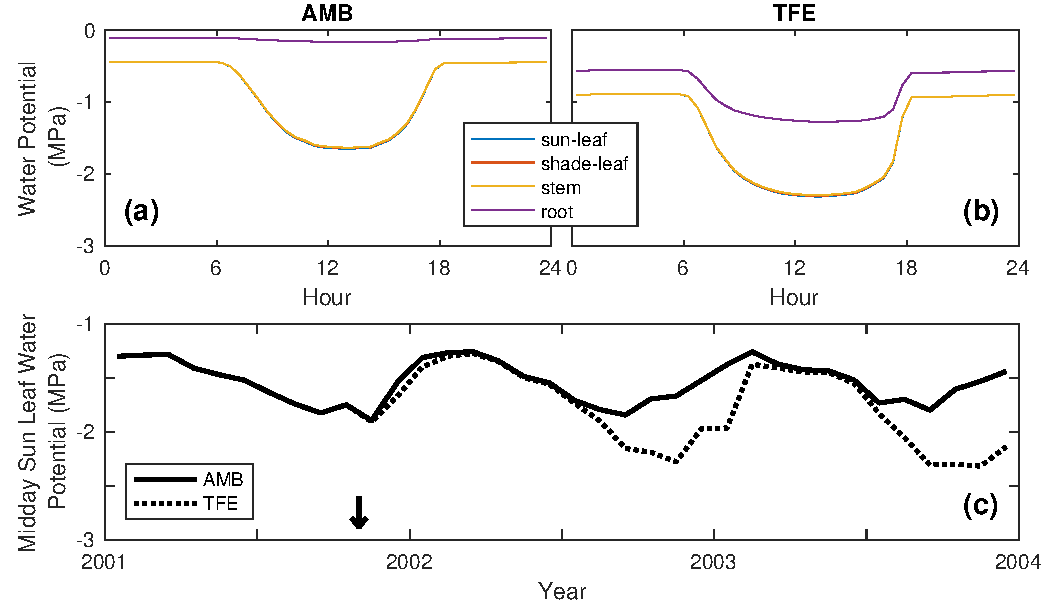
\includegraphics[width=30pc]{../figs3/vwp.pdf}
     \caption{Modeled vegetation water potential at  Caxiuan\~a, Brazil.
     (a) 2003 dry season (SON) diurnal mean, ambient through-fall conditions,
     (b) 2003 dry season diurnal mean, with 60\% TFE.
     Curves are drawn for sunlit leaf, shaded leaf, stem, and root water potentials, with the latter three overlapping.
     (c) Monthly average midday (12h-14h) root and leaf water potential, under ambient (solid line) and TFE (dotted line) conditions.
     Note that TFE begins Nov 1, 2001, as indicated by the vertical arrow. 
     }
     \label{fig:vwp}
  \end{figure}

  
    \clearpage
    \begin{figure}[h]
     \centering
     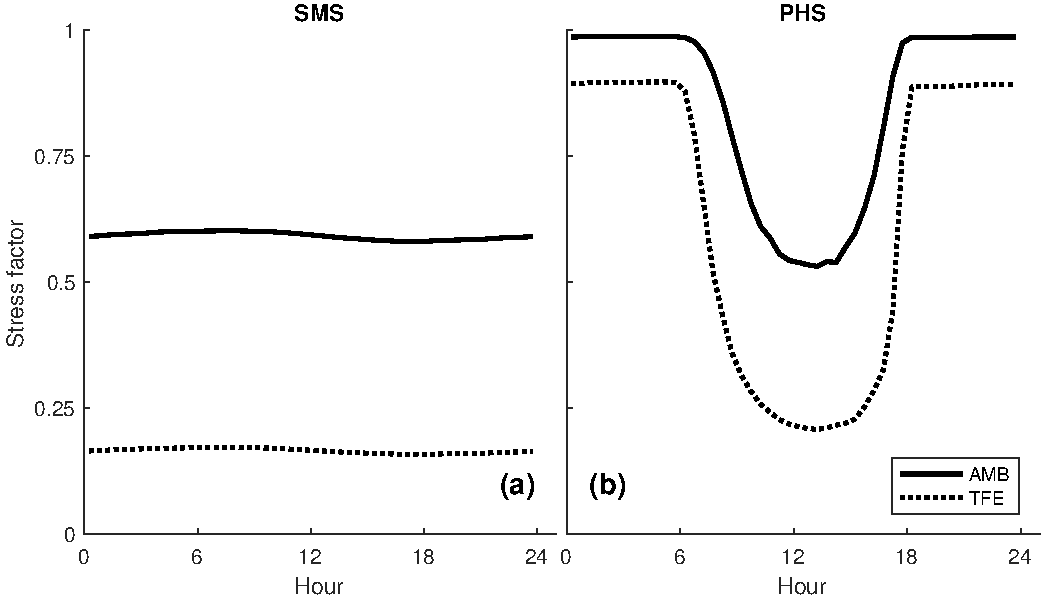
\includegraphics[width=30pc]{../figs3/fig4.pdf}
     \caption{2003 dry season (SON) diurnal mean water stress function for 
     (a) SMS, and
     (b) PHS.
     Note that the water stress factor equals 1 when there is no stress and 0 when fully stressed.
     }
     \label{fig:stress1}
  \end{figure}
  
      \clearpage
    \begin{figure}[h]
     \centering
     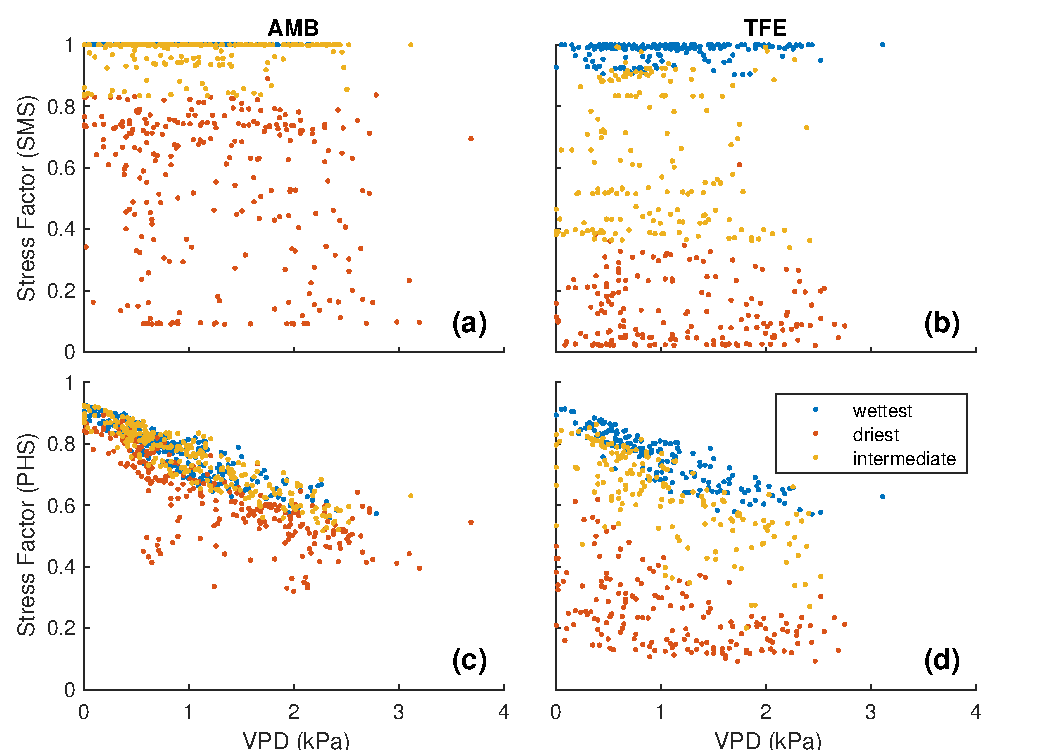
\includegraphics[width=30pc]{../figs3/vpdstress.pdf}
     \caption{Water stress factor versus vapor pressure deficit (2002-2003), for timesteps with downwelling shortwave radiation between 400 and 425 W/m2 (n=515).
     Radiation is controlled to highlight the relationship with VPD, the reverse (controlling for VPD) is shown in Figure \ref{supp:fsds}.
     For SMS (a,b), data are subdivided based on average soil matric potential, weighted by root fraction.
     For PHS (c,d), data are subdivided based on predawn (5h) root water potential.
     Blue dots represent the wettest tercile, yellow dots represent the intermediate tercile, and red dots represent the driest tercile (see Table \ref{tab:tercile}).
     }
     \label{fig:stress2}
       \end{figure}
      
          \clearpage   
  \begin{figure}[h]
     \centering
     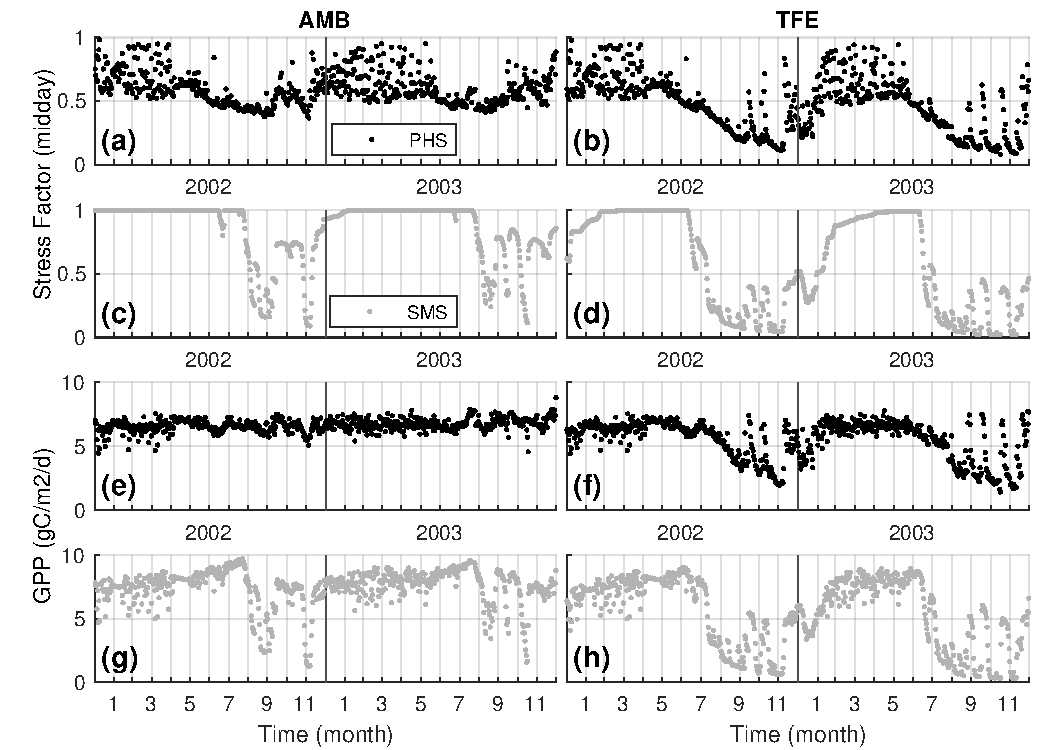
\includegraphics[width=30pc]{../figs3/gpp.pdf}
     \caption{Daily stress factor (midday, averaged over 12h-14h) and GPP during 2002-2003 under ambient (left) and TFE (right) conditions.
     Output from the SMS configuration (a,b,e,f) are plotted with gray color, while output from the PHS configuration (c,d,g,h) are plotted in black.
     }
     \label{fig:gpp}
  \end{figure} 
         
  \clearpage   
  \begin{figure}[h]
     \centering
     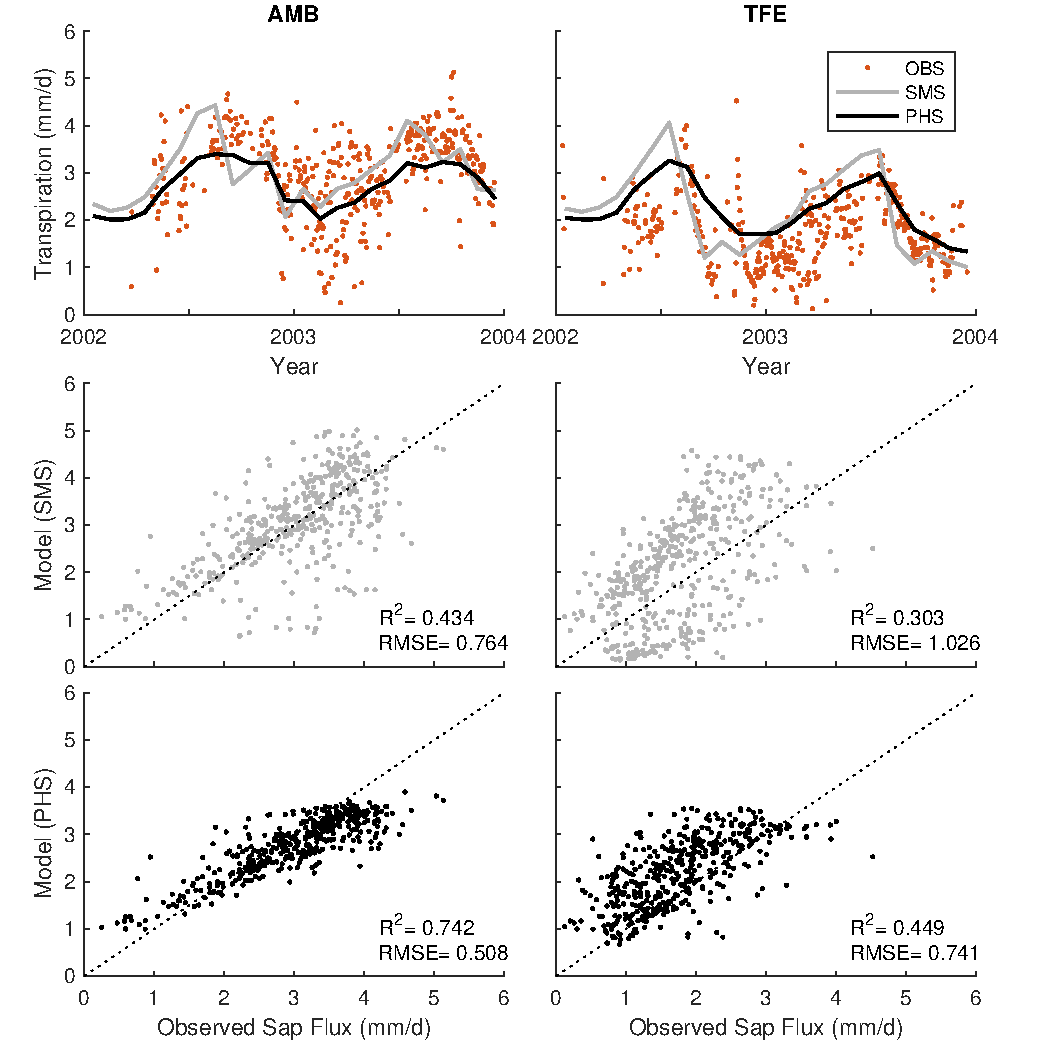
\includegraphics[width=30pc]{../figs3/T.pdf}
     \caption{(a,b) Monthly mean water stress function. The water stress factor equals 1 when there is no stress and 0 when fully stressed.
     (c,d) Monthly mean transpiration (W/m$^2$).
     (e,f) Monthly mean gross primary productivity (g/m$^2$/d). 
     Solid lines correspond to ambient through-fall conditions, and dotted lines feature 60\% through-fall exclusion.
     Black lines represent model output.
     Red lines show observational transpiration derived from sap flux (see zqz).
     PHS is on for (a), (c), and (e). PHS is off for (b), (d), and (f).
     }
     \label{fig:t}
  \end{figure}

  \begin{figure}[h]
     \centering
     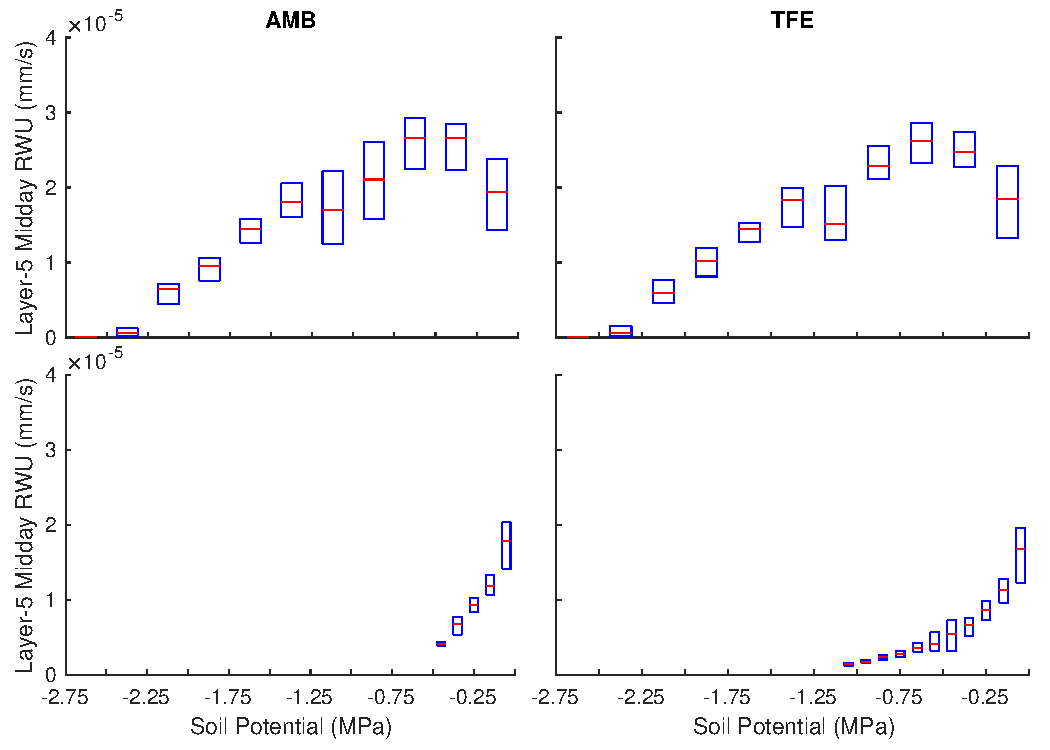
\includegraphics[width=30pc]{../figs3/rwu.pdf}
     \caption{Binned boxplot of root water uptake versus soil potential for Soil Layer 5 (2002-3).
     Red lines mark the median, with boxes spanning the interquartile range.
     Bin sizes are 0.25 MPa for SMS and 0.1 MPa for PHS.
     Soil Layer 5 is shown, because it is near the surface (20 to 32 cm) and has a large root fraction (14.4\%).
     Only midday (12h-14h) timesteps are shown to highlight the relationship with soil potential.}
     \label{fig:rwu}
  \end{figure}
  \clearpage
  

        \clearpage
    \begin{figure}[h]
     \centering
     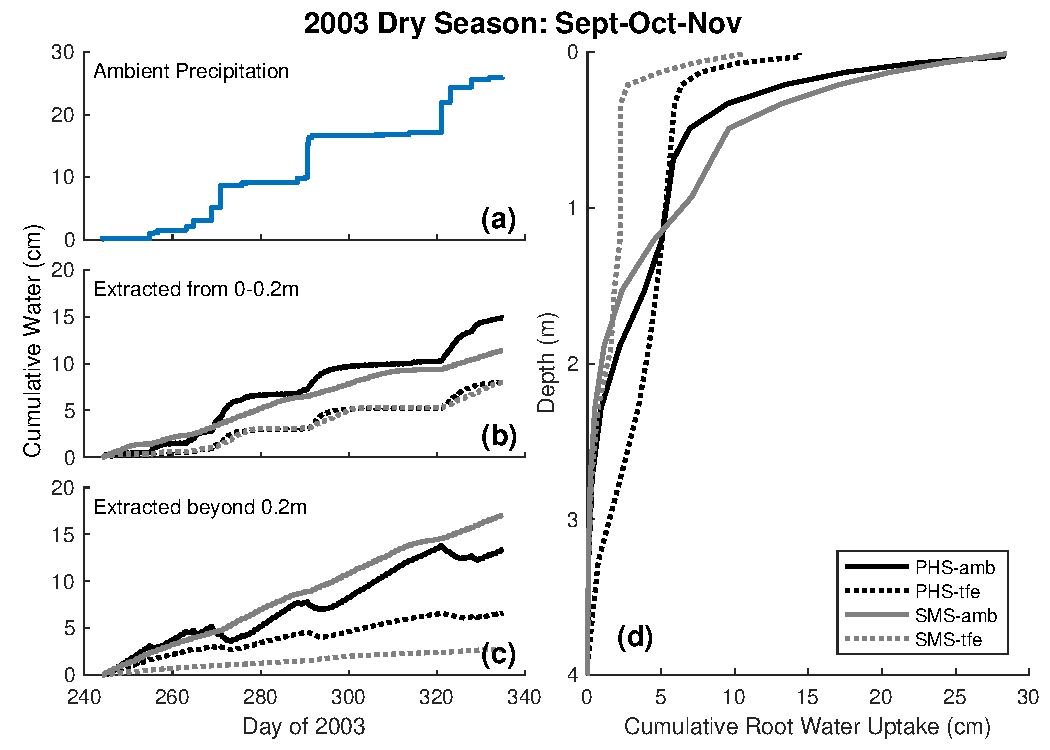
\includegraphics[width=30pc]{../figs3/qdry.pdf}
     \caption{2003 dry season (SON) cumulative root water uptake and precipitation. 
     (a) Cumulative root water uptake with depth across the four simulations.
     (b,c) Cumulative water uptake over time from above and below 0.2m, respectively.
     (d) Cumulative precipitation under ambient conditions.
     }
     \label{fig:qdry}
  \end{figure}
  
        \clearpage
    \begin{figure}[h]
     \centering
     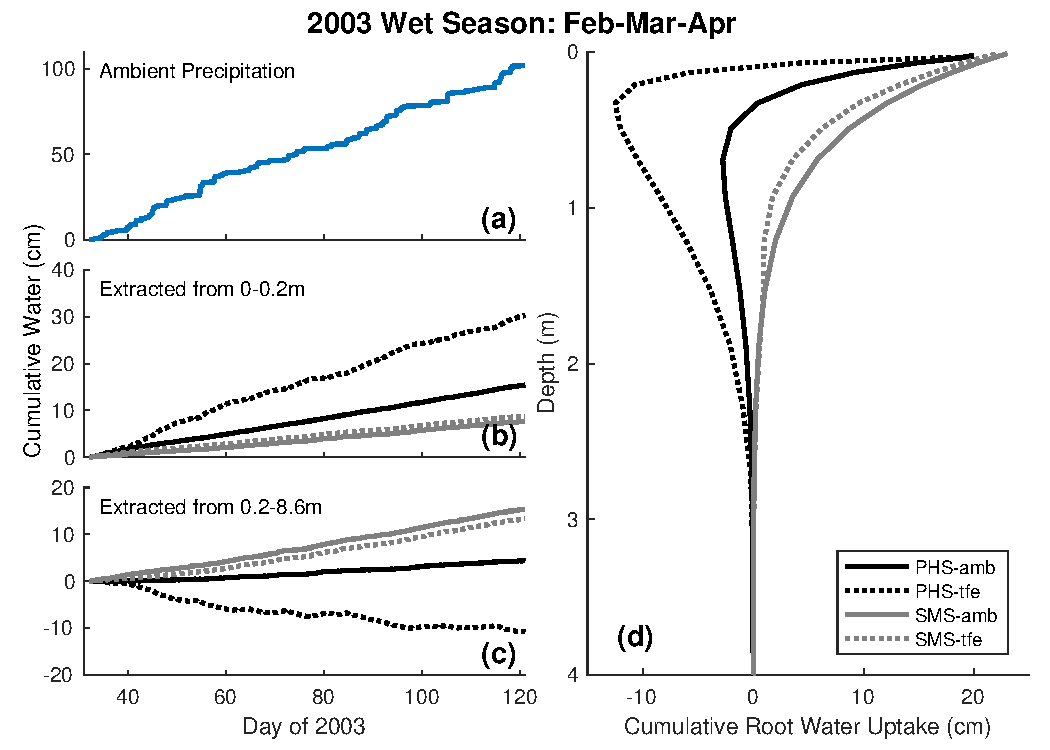
\includegraphics[width=30pc]{../figs3/qwet.pdf}
     \caption{2003 wet season (FMA) cumulative root water uptake and precipitation. 
     (a) Cumulative root water uptake with depth across the four simulations.
     (b,c) Cumulative water uptake over time from above and below 0.2m, respectively.
     (d) Cumulative precipitation under ambient conditions.
     }
     \label{fig:qwet}
  \end{figure}
  
    \clearpage
    \begin{figure}[h]
     \centering
     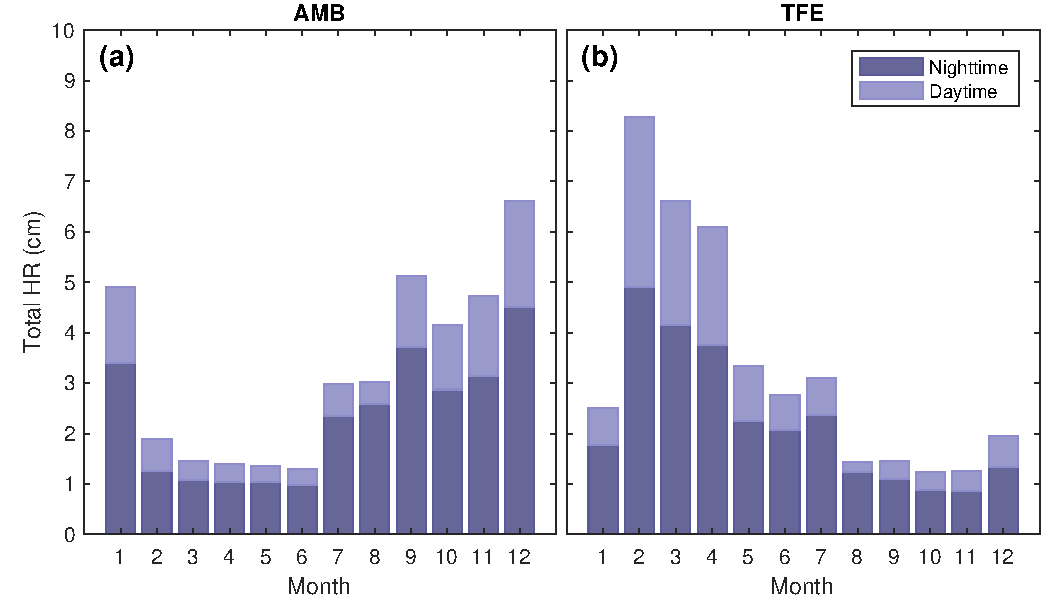
\includegraphics[width=30pc]{../figs3/hr.pdf}
     \caption{Total hydraulic redistribution (cm) by month across in 2003. For (a) ambient through-fall conditions, and (b) 60\% through-fall exclusion. 
     Darker shading shows portion of HR at night [6pm,6am), lighter shading shows portion of HR during day [6am,6pm).
     Total HR refers to the sum of all negative root water uptake flows, where water is deposited by roots into a given soil layer.}
     \label{fig:hr}
  \end{figure}

  
      \clearpage
    \begin{figure}[h]
     \centering
     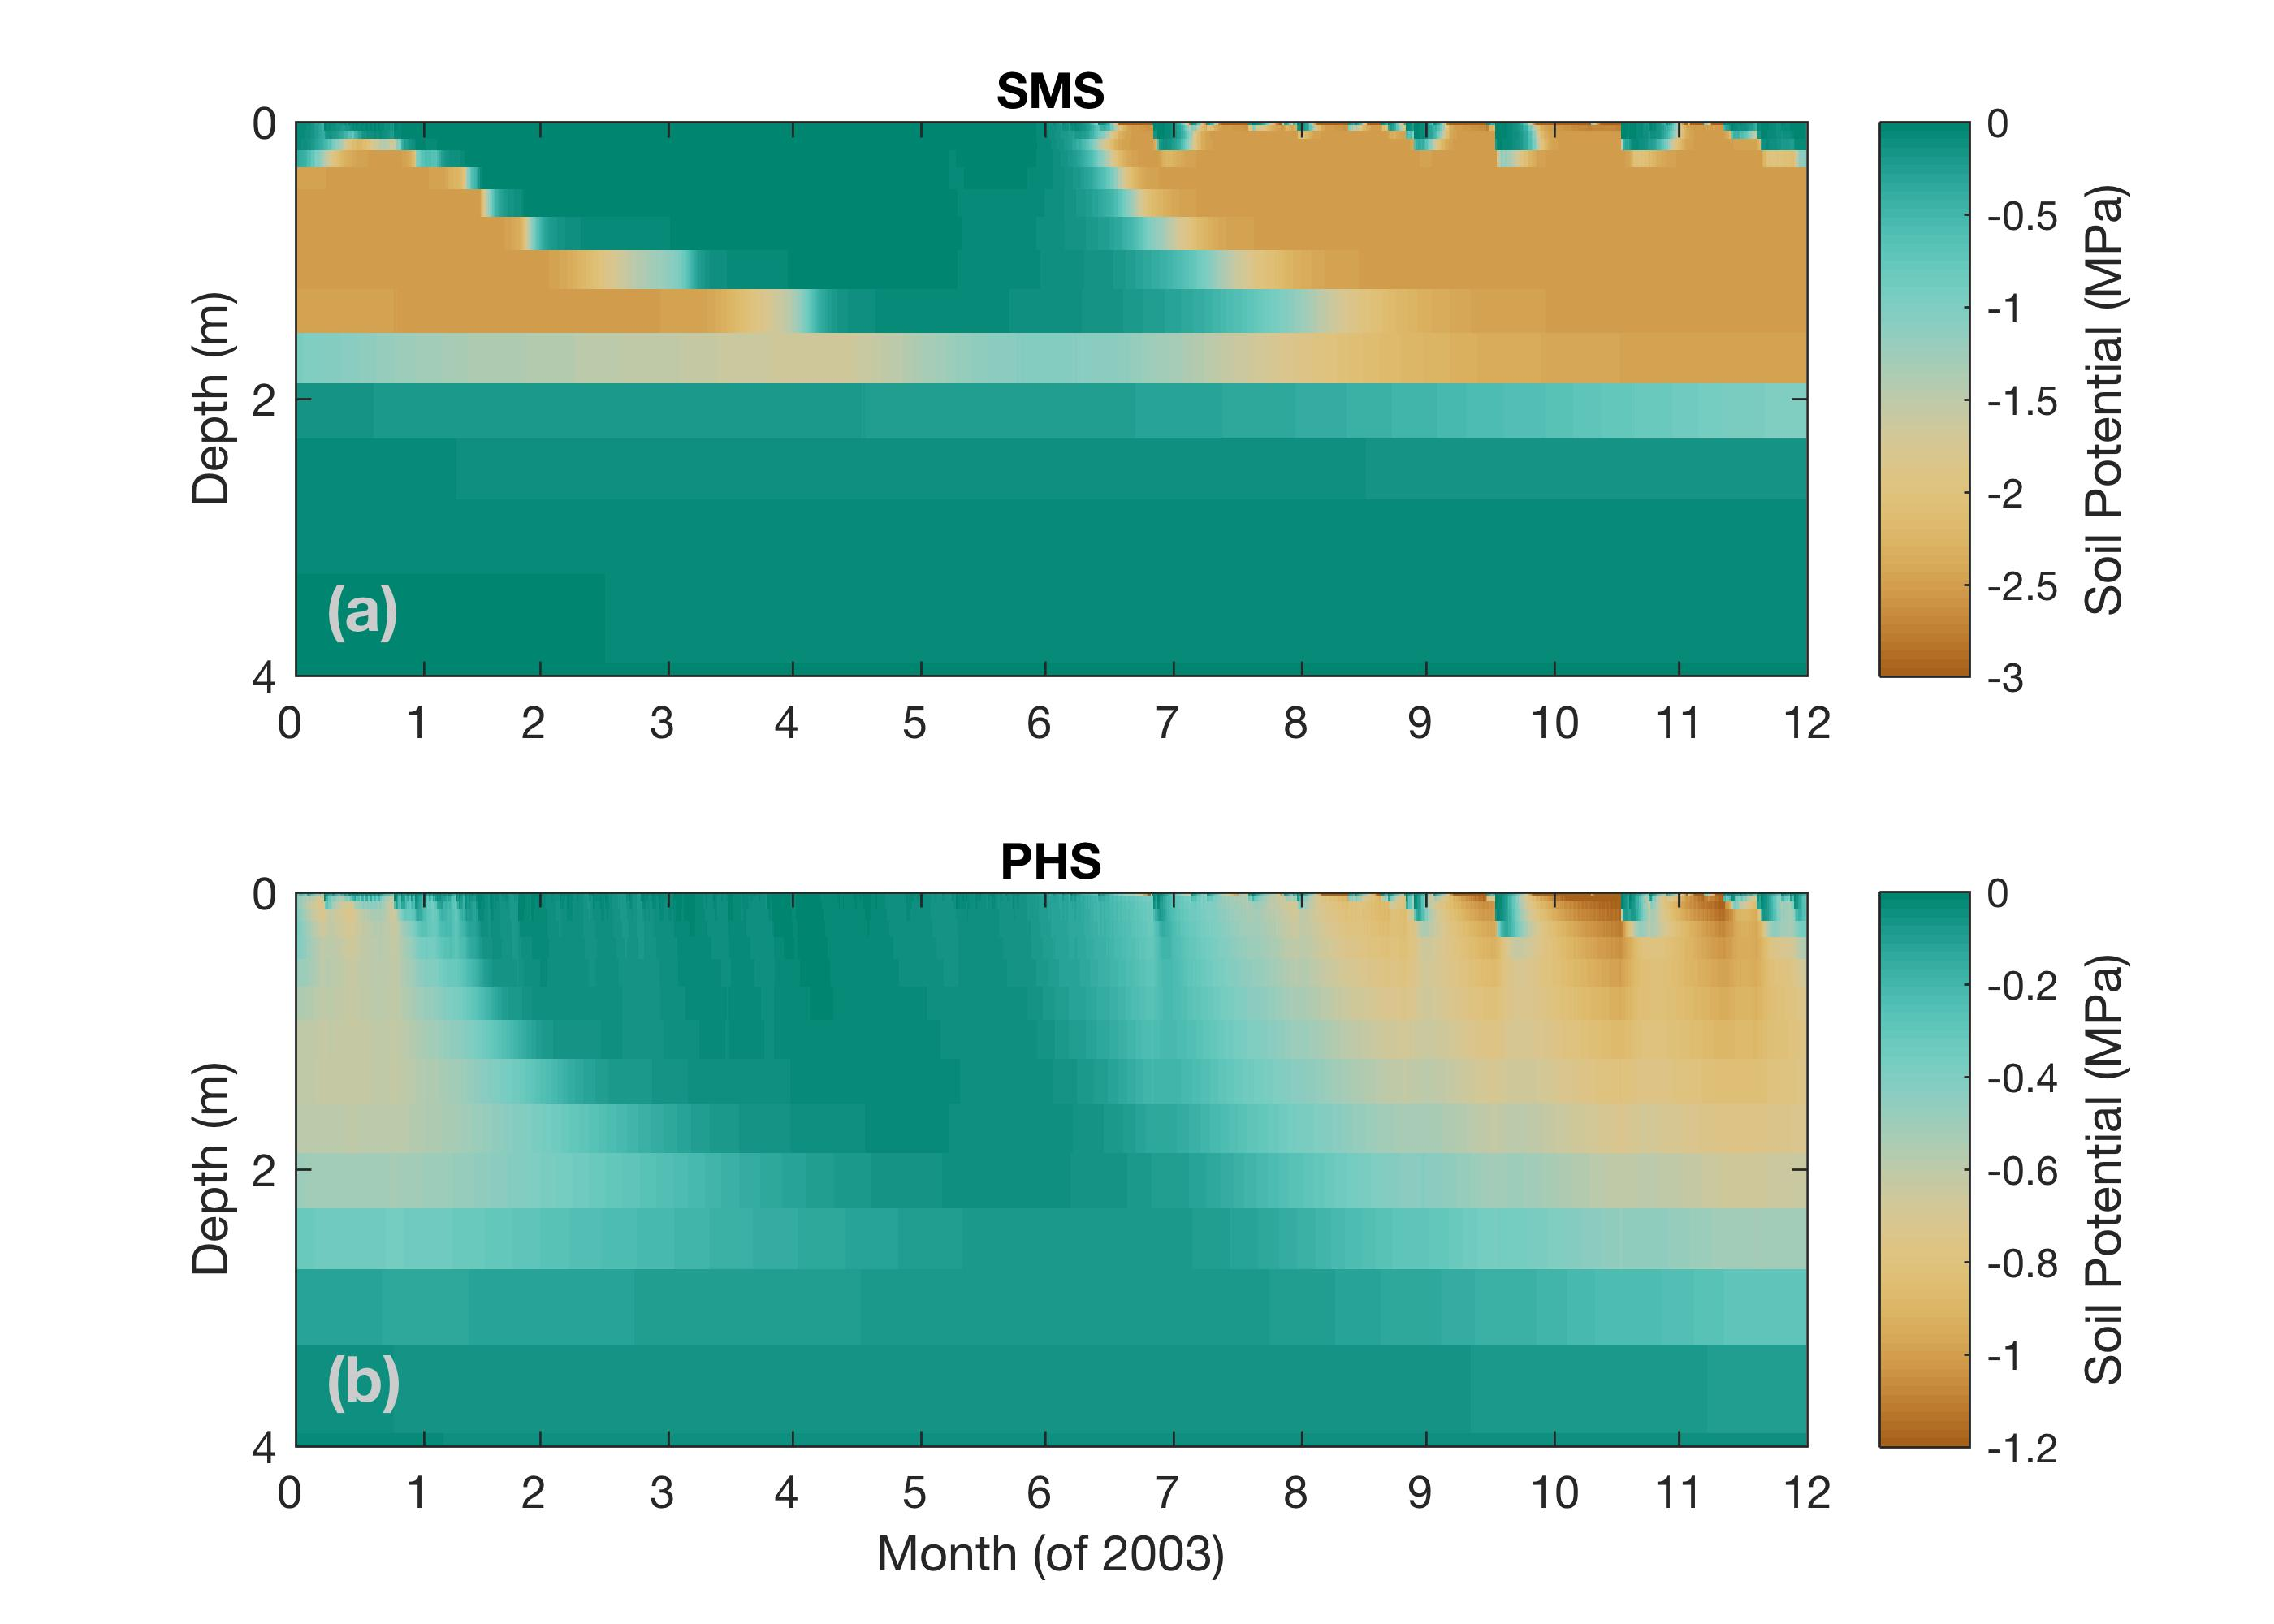
\includegraphics[width=30pc]{../figs3/smp.jpg}
     \caption{Vertical profile of soil water potential (MPa) over time under 60\% through-fall exclusion, for
     (a) SMS, and 
     (b) PHS.
     Note that color axes are different.
     SMS soil potential spends long periods at -2.5MPa, which is the value of parameter $\psi_c$.
     Figure \ref{fig:sm2} subsets this data at 0.5m depth (dotted line), plotted alongside observations.
     Soil potential under ambient conditions is shown in Supp Fig \ref{supp:sm}.
 }
     \label{fig:sm}
  \end{figure}
  
        \clearpage
    \begin{figure}[h]
     \centering
     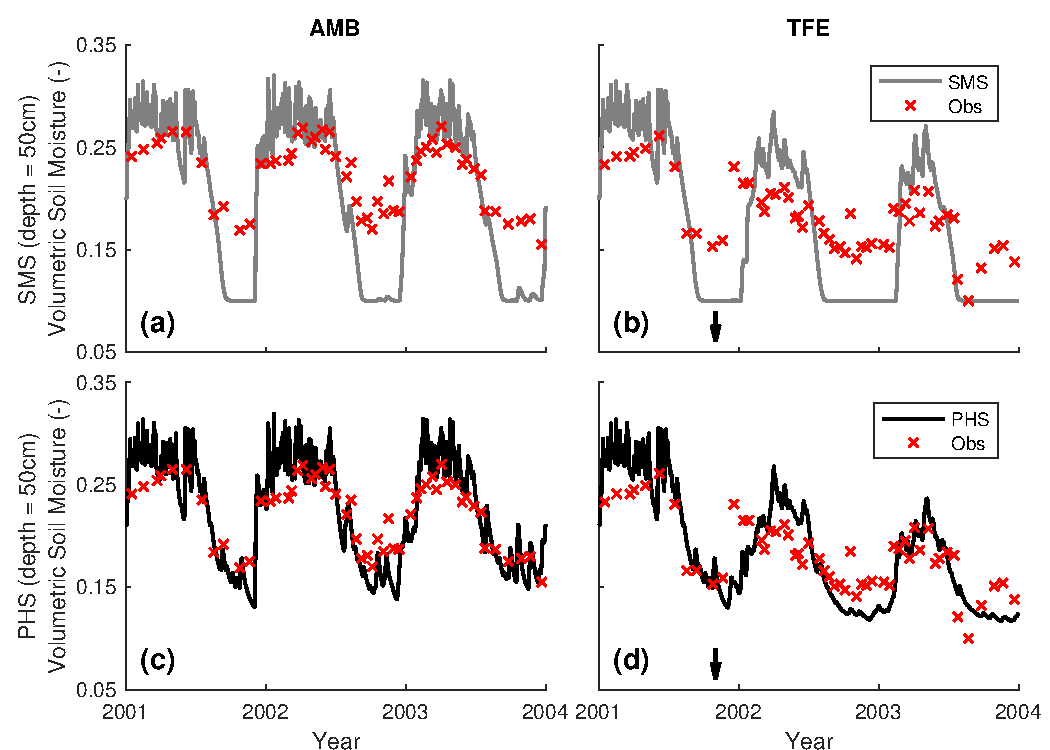
\includegraphics[width=30pc]{../figs3/sm2.pdf}
     \caption{Volumetric soil moisture (-) over time under ambient and TFE conditions at depth of 50cm.
     (a/b) SMS
     (c/d) PHS.
     RMSE are 0.048, 0.049, 0.022, and 0.029.
     Arrows indicate start of TFE. Figure \ref{supp:sm2} shows the same plots at 7 other soil depths. }
     \label{fig:sm2}
  \end{figure}

              \begin{figure}[h]
     \centering
     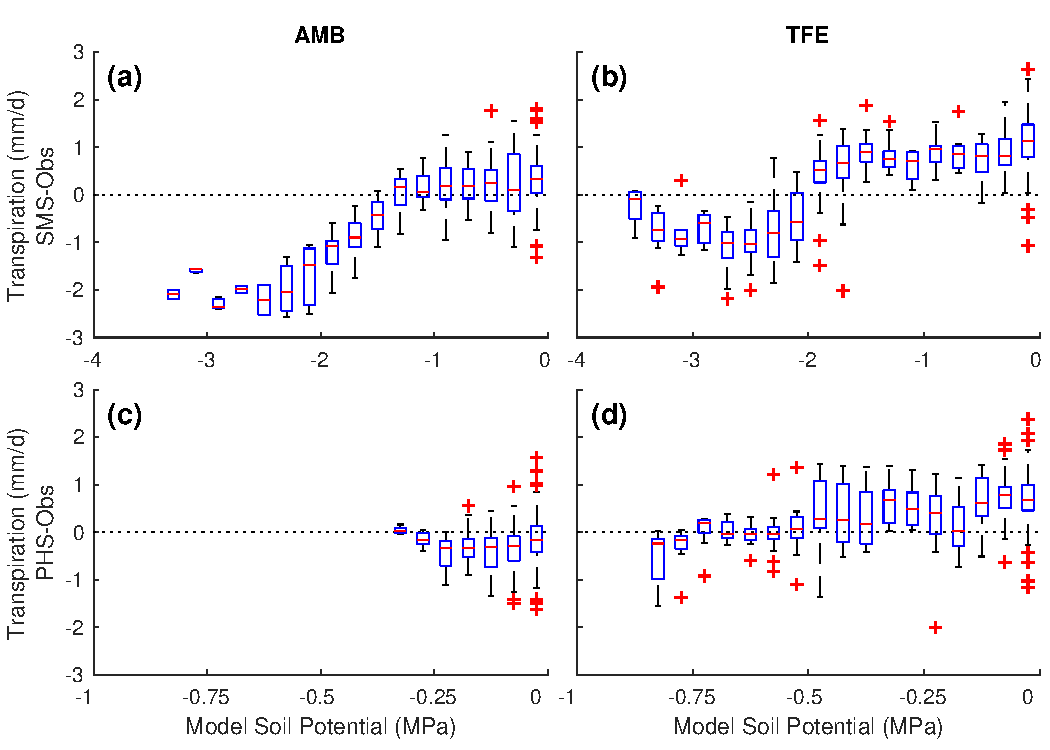
\includegraphics[width=30pc]{../figs3/sm3.pdf}
     \caption{Binned boxplot showing the difference between modeled and observed transpiration (mm/d) versus model soil potential.
     Red lines are drawn at the median, with boxes spanning the interquartile range.
     The two models use different root water uptake paradigms, from which we define different operators for column effective soil potential.
     For SMS we average over the soil column weighted by root fraction and over time (daily mean).
     For PHS we use predawn (5h) root water potential.
     Bin widths are 0.2 MPa for SMS (a,b) and 0.05 MPa for PHS (c,d).
}
     \label{fig:cool}
  \end{figure}
          \clearpage

\clearpage

\appendix
%====================
%  APPENDIX
%====================

\section{Supplementary Figures}


      \begin{figure}[h]
     \centering
     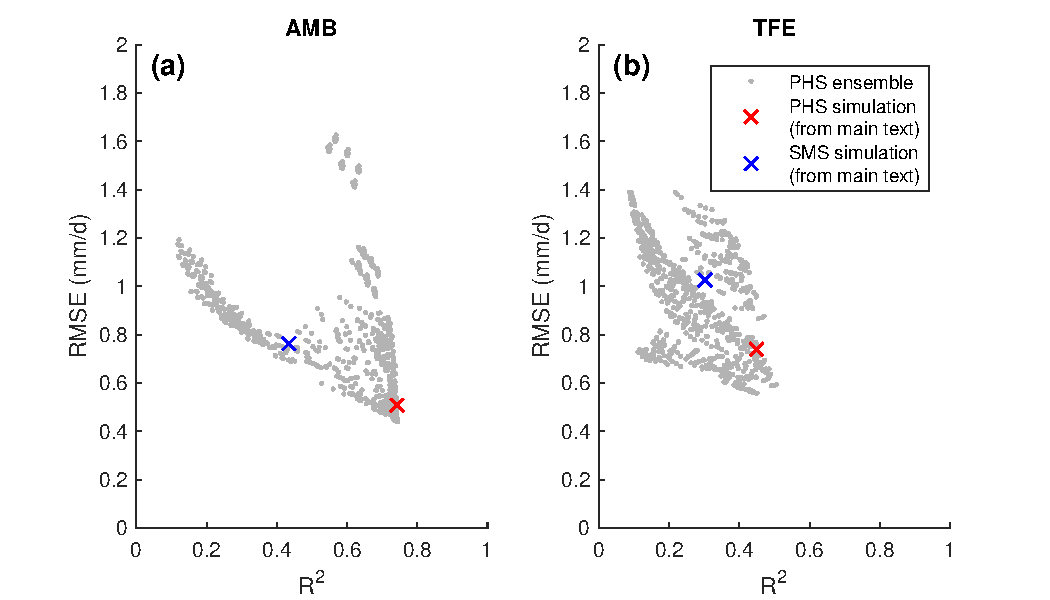
\includegraphics[width=30pc]{../figs3/ens.pdf}
     \caption{Parameter tuning exercise.
     }
     \label{supp:ens}
       \end{figure}
         \clearpage

      \begin{figure}[h]
     \centering
     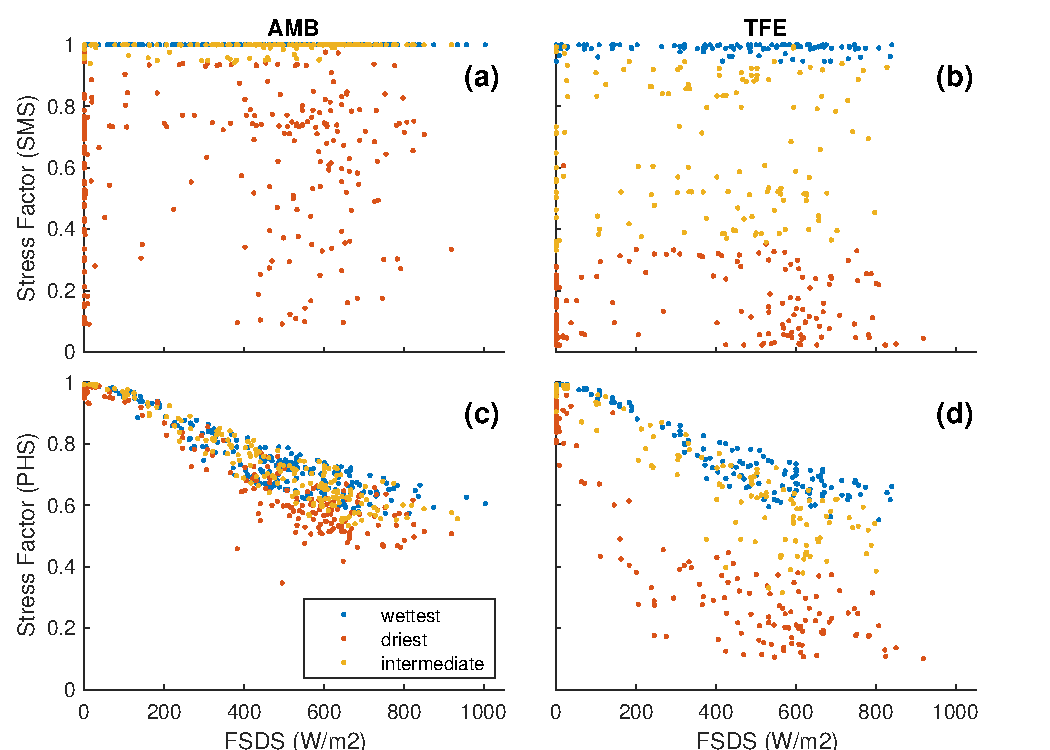
\includegraphics[width=30pc]{../figs3/suppstress.pdf}
     \caption{Water stress factor versus downwelling shortwave radiation (2002-2003), for timesteps with VPD between 1 and 1.0559 kPa (n=470).
     VPD is controlled to highlight the relationship with downwelling radiation, the reverse (controlling for radiation) is shown in Figure \ref{fig:stress2}.
     For SMS (a,b), data are subdivided based on average soil matric potential, weighted by root fraction.
     For PHS (c,d), data are subdivided based on predawn (5h) root water potential.
     Blue dots represent the wettest tercile, yellow dots represent the intermediate tercile, and red dots represent the driest tercile.
     }
     \label{supp:fsds}
       \end{figure}
         \clearpage

  
  \begin{figure}[h]
     \centering
     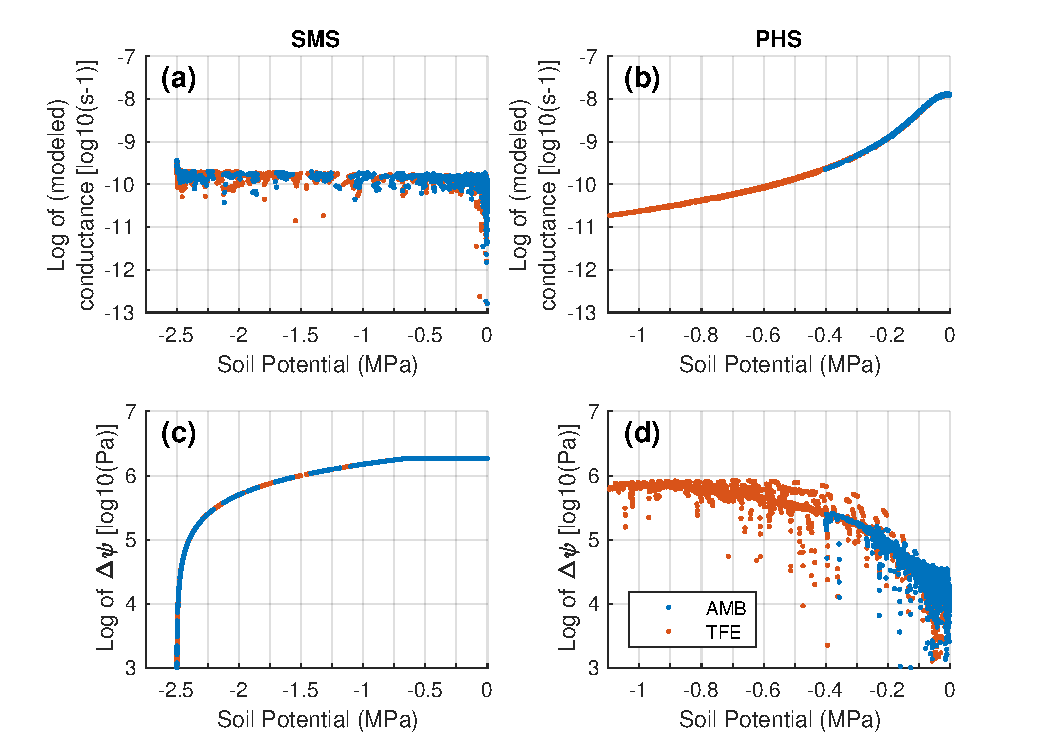
\includegraphics[width=30pc]{../figs3/suppcond.pdf}
     \caption{Log of conductance versus soil potential for Soil Layer 5 (2002-3).
     Only midday (12h-14h) timesteps are shown to emphasize the relationship with soil potential.
     With SMS, conductance is not modeled explicitly, but rather calculated as $k$=$q/\Delta\psi$ (see Section zqz). 
     Beyond 2.5MPa, SMS implied conductance equals 0.
     PHS conductance captures both root tissue and soil matrix resistances (operating in series).}
     \label{supp:cond}
  \end{figure}
  \clearpage

\clearpage   
  \begin{figure}[h]
     \centering
     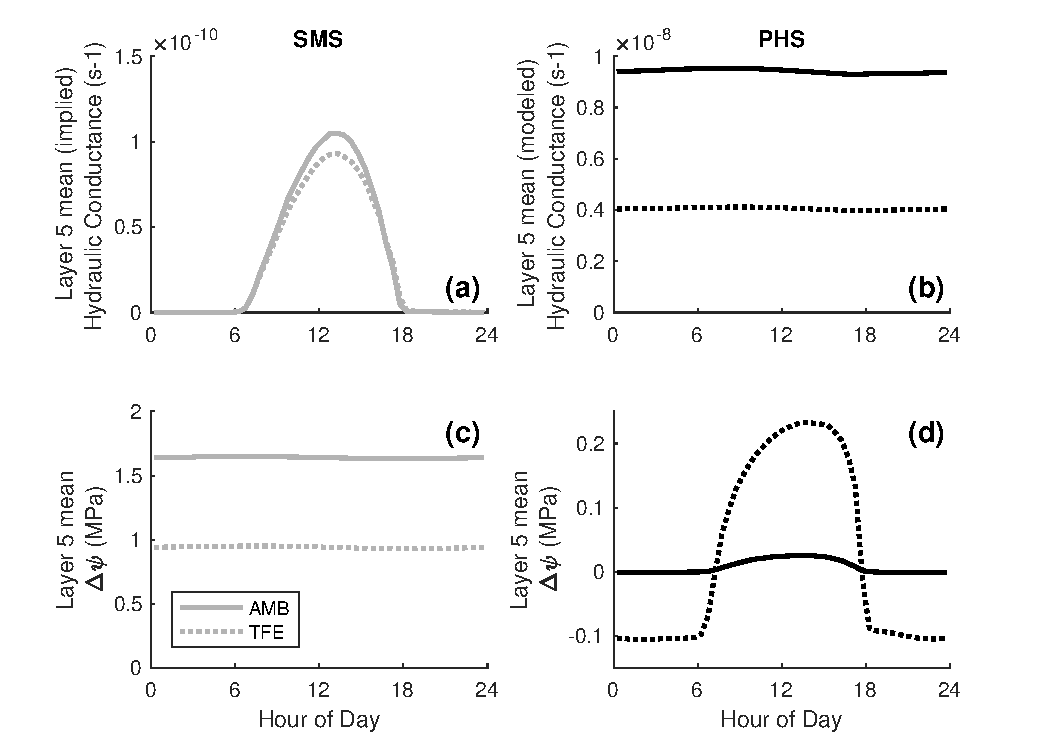
\includegraphics[width=30pc]{../figs3/k.pdf}
     \caption{2003 diurnal mean of Soil Layer 5 conductance and $\Delta\psi$, under ambient and TFE conditions. 
     }
     \label{supp:cond2}
  \end{figure}
  
      \begin{figure}[h]
     \centering
     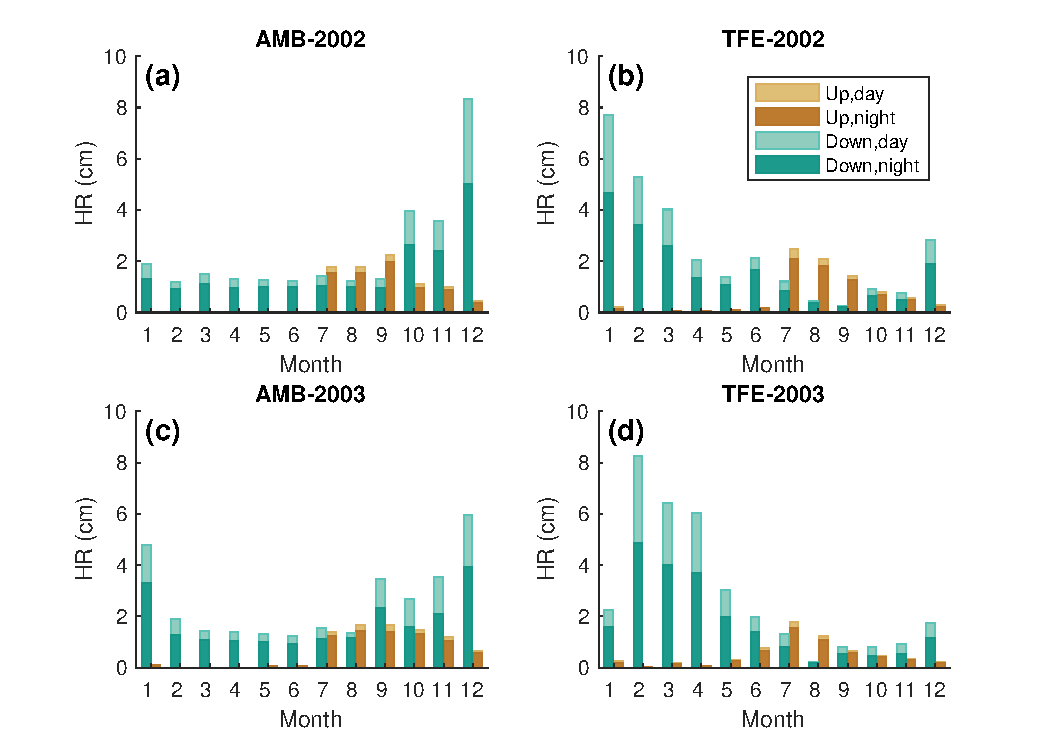
\includegraphics[width=30pc]{../figs3/hr2}
     \caption{PHS hydraulic distribution during 2003. Alternative version partitioning by direction.}
     \label{supp:hr}
  \end{figure}
  \clearpage

  
        \clearpage
    \begin{figure}[h]
     \centering
     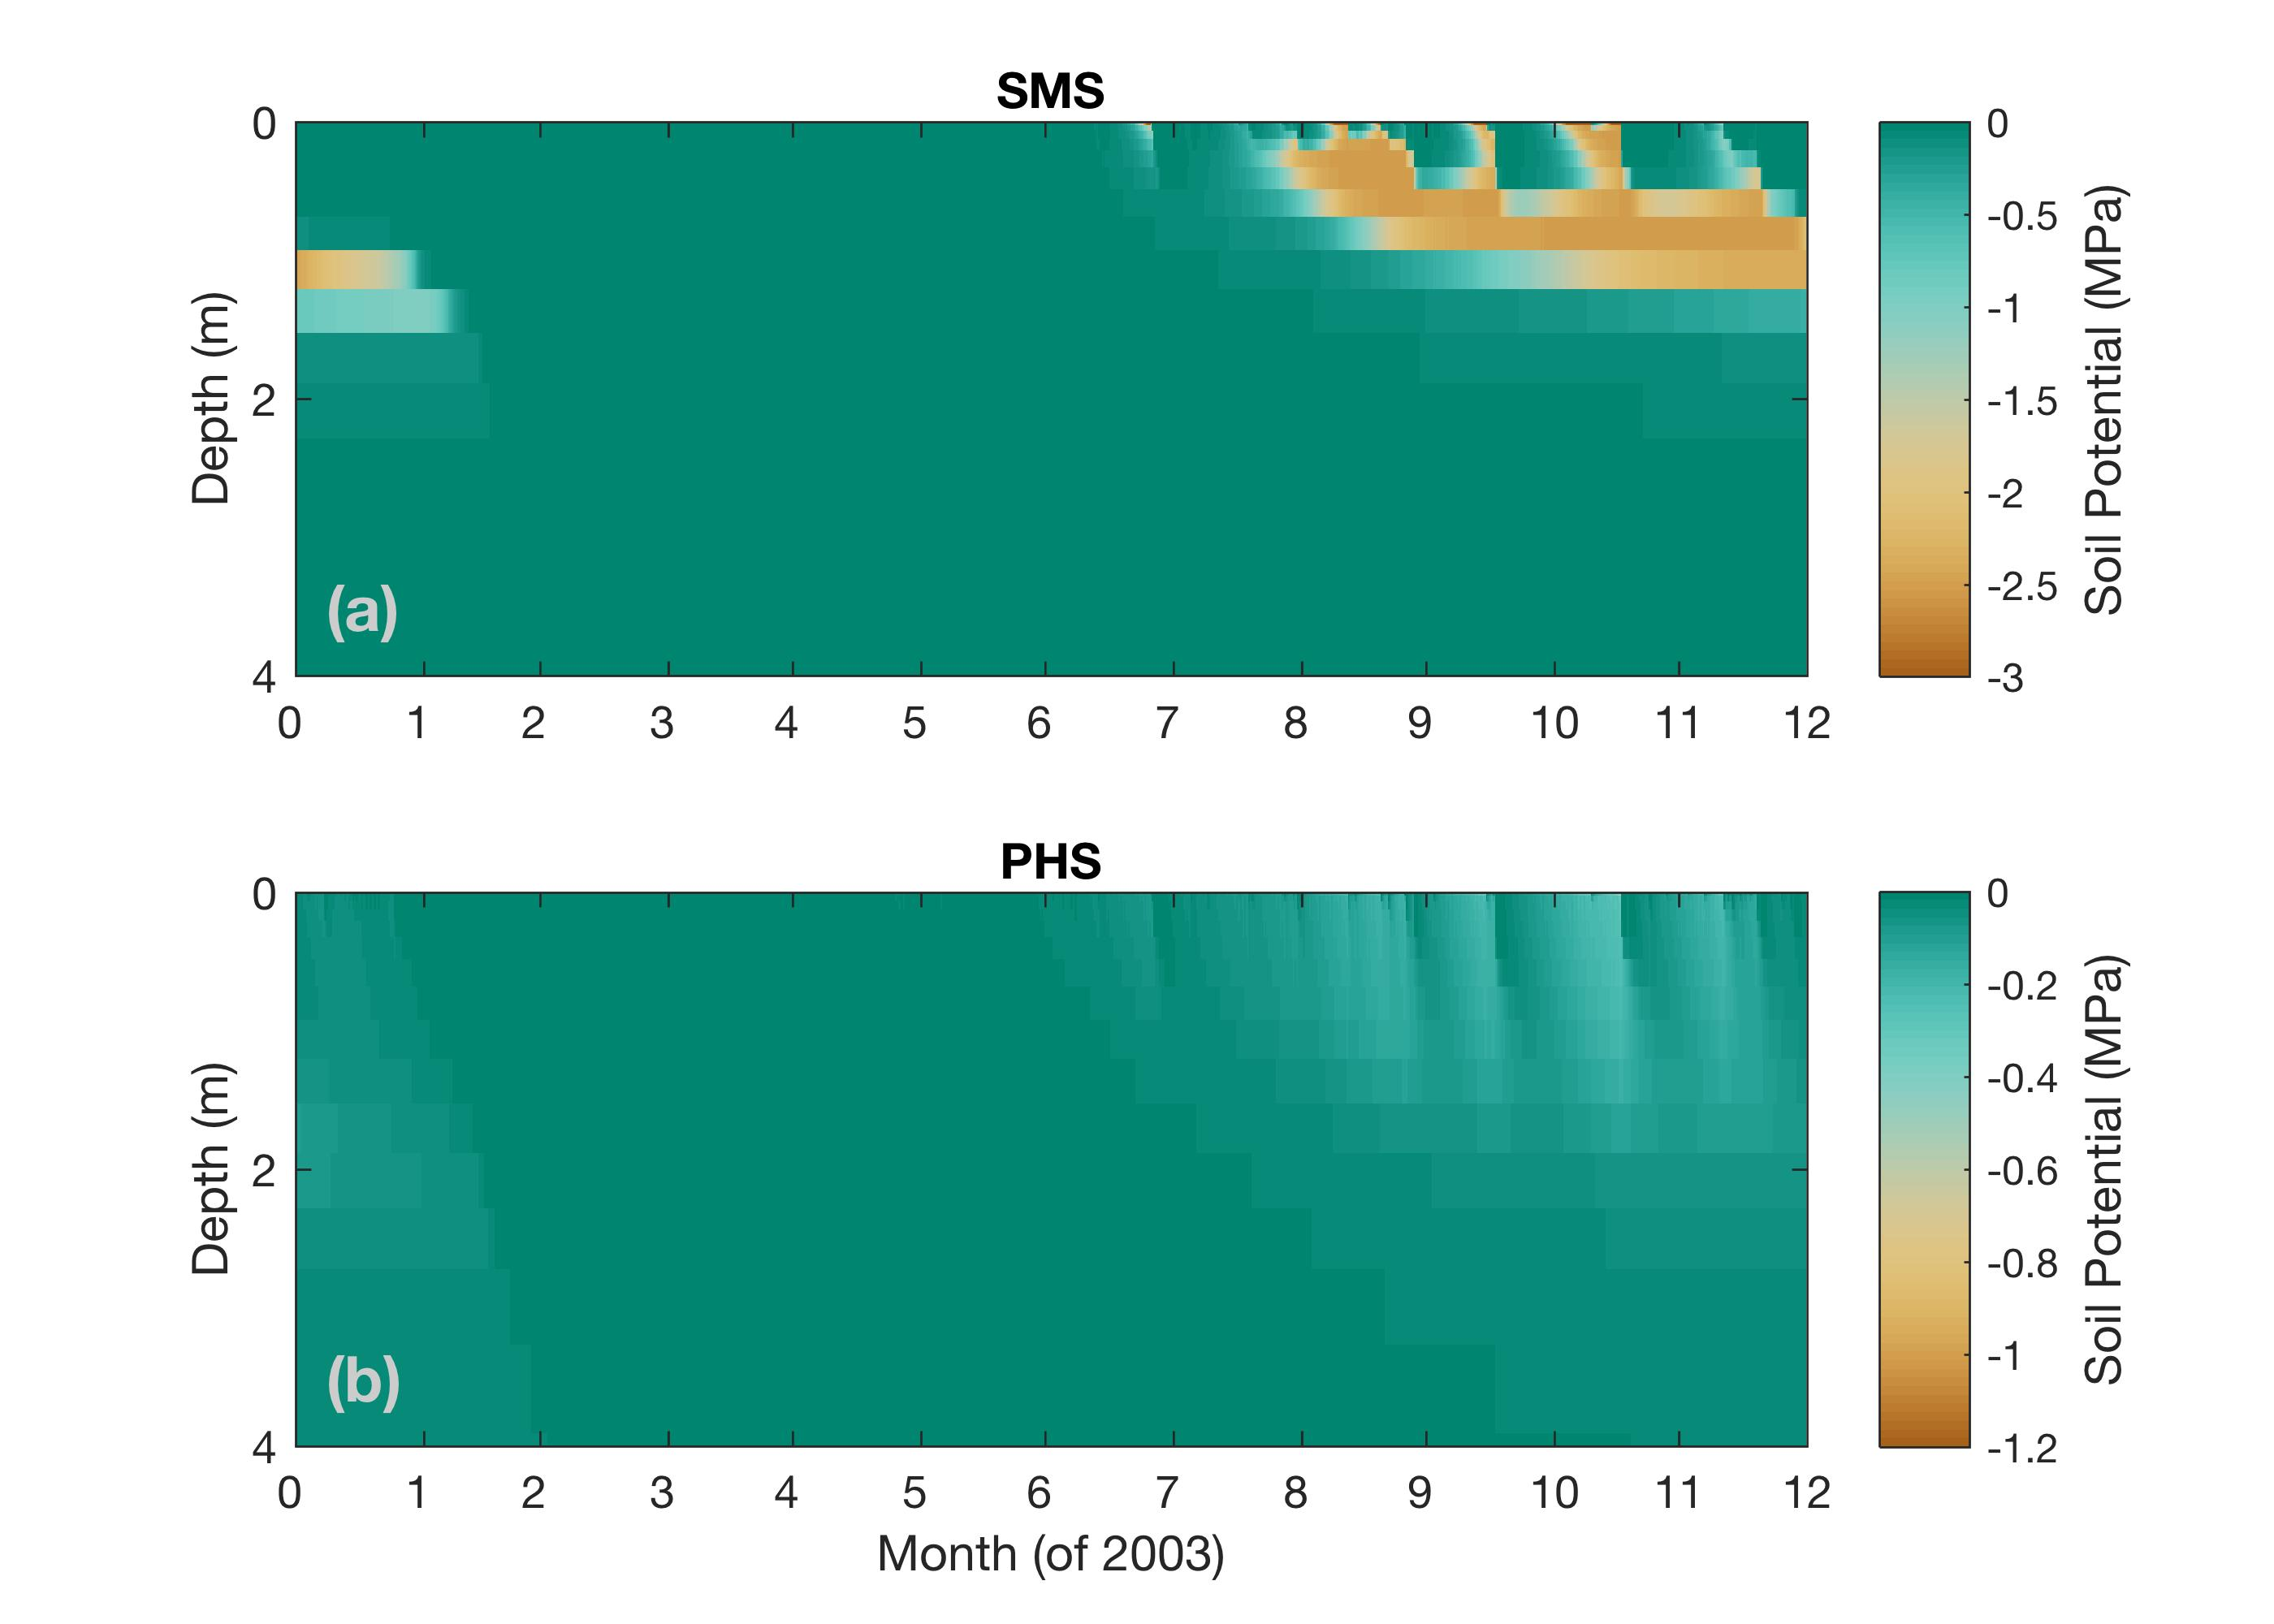
\includegraphics[width=30pc]{../figs3/suppsmp.jpg}
     \caption{Vertical profile of soil water potential (MPa) through time under ambient through-fall conditions, for
     (a) PHS, and 
     (b) SMS.
     Note that color axes are different. }
     \label{supp:sm}
  \end{figure}
  

    \begin{figure}[h]
     \centering
     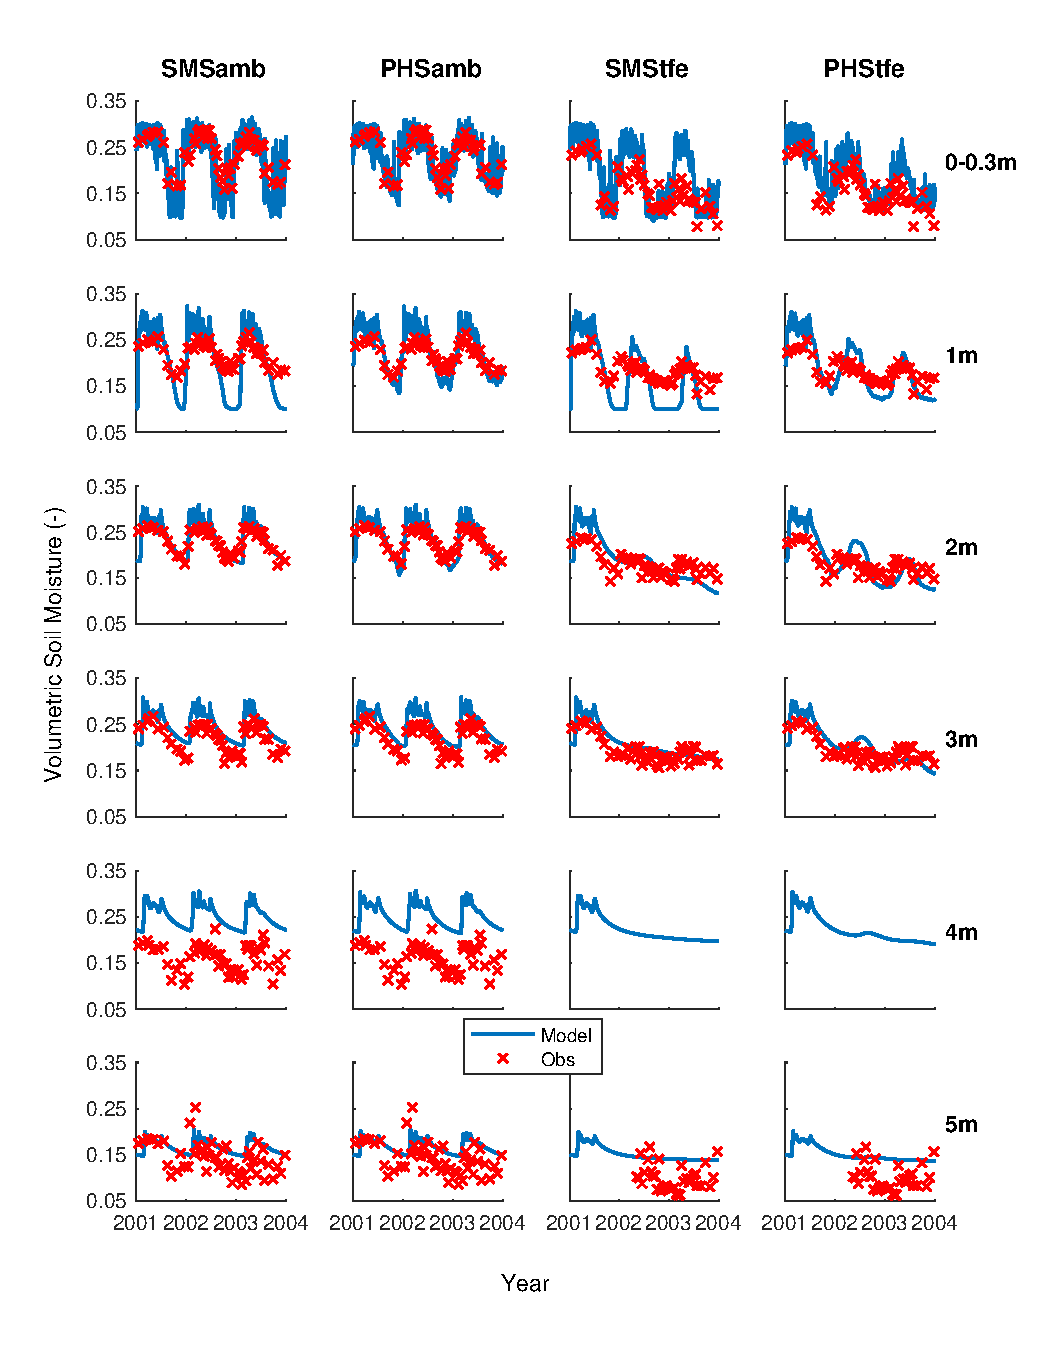
\includegraphics[width=30pc]{../figs3/suppsm2.pdf}
     \caption{Time series of soil moisture by soil layer.
     Complements Figure \ref{fig:sm}}
     \label{supp:sm2}
  \end{figure}
          \clearpage
          
     \begin{figure}[h]
     \centering
     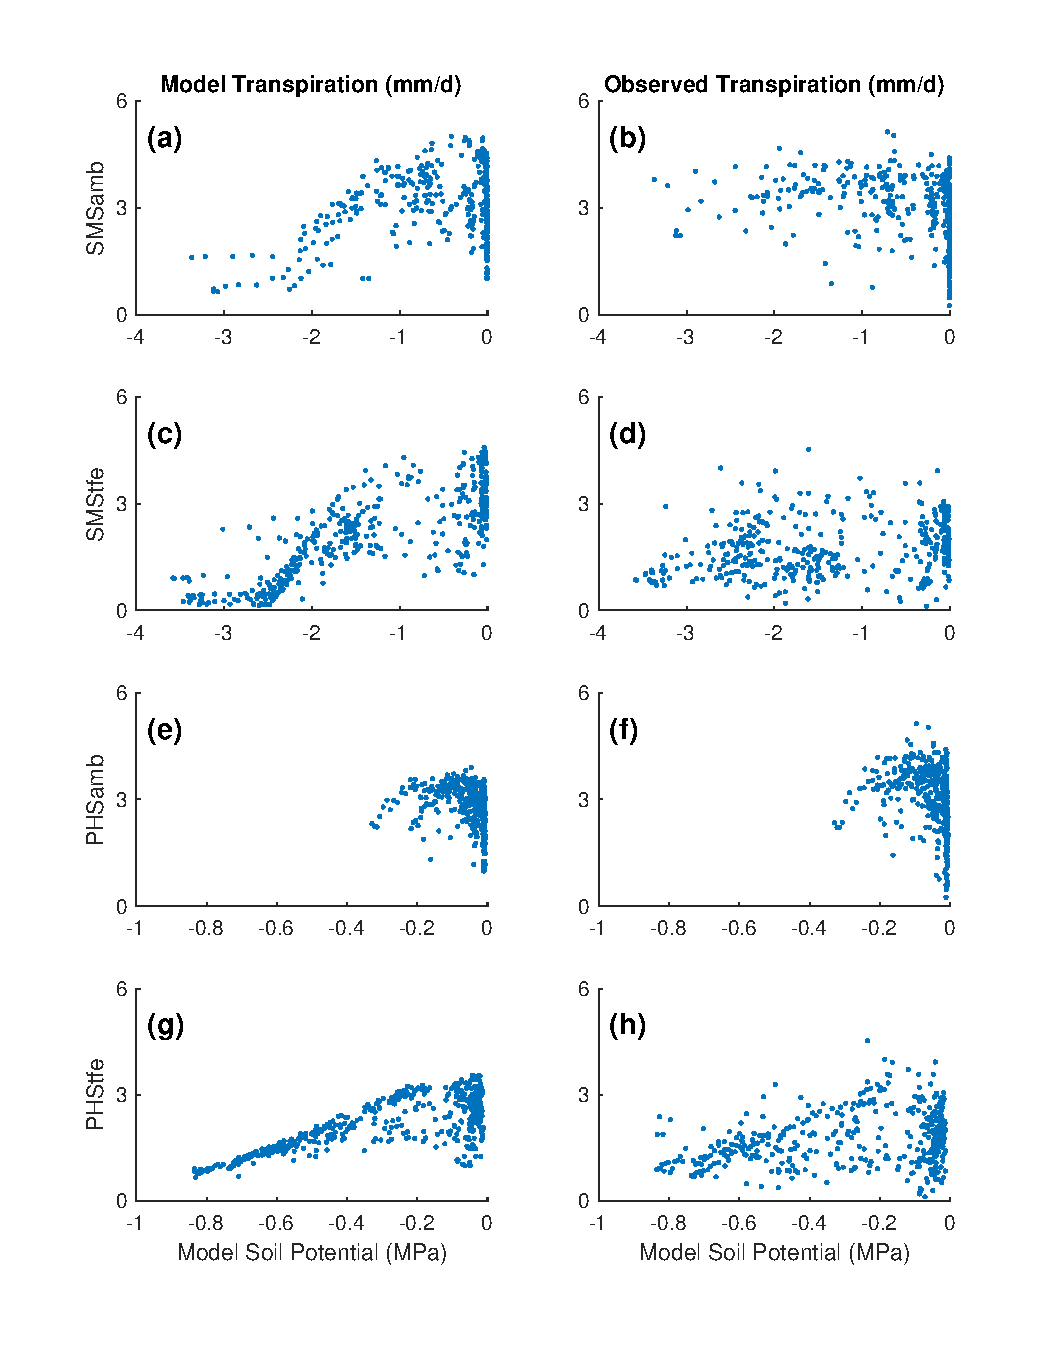
\includegraphics[width=30pc]{../figs3/suppcool.pdf}
     \caption{Modeled (left column) and observed (right column) transpiration  vs. model soil potential.
     Complements Figure \ref{fig:cool}}
     \label{supp:cool}
  \end{figure}
          \clearpage
          



\section{Appendix to Model Description}

% Details on water supply
\subsection{Details of Water Supply}

PHS resolves flow across four different segments, soil-to-root, root-to-stem, stem-to-leaf, and leaf-to-transpiration.

Stem-to-leaf. The area bases are sunlit and shaded leaf area, respectively. 
Note that gravity is assumed negligible here. 
Likewise there is no length scaling applied to maximum conductance. 
Therefore the input parameters for $k_{1,\text{max}}$ should be conductances ($s^{-1}$).

\begin{linenomath*} \begin{equation} \begin{aligned}
q_{1a} &= k_{1} \cdot \text{LAI-sun}  \cdot \left( \psi_{\text{stem}}-\psi_{\text{sun-leaf}}\right) \\
q_{1b} &= k_{1} \cdot \text{LAI-shade} \cdot  \left( \psi_{\text{stem}}-\psi_{\text{shade-leaf}}\right)
\end{aligned} \end{equation} \end{linenomath*}

\begin{linenomath*} \begin{equation}
k_{1} = k_{1,\text{max}} \cdot f\left(\psi_{\text{stem}}\right)
\end{equation} \end{linenomath*}

\begin{linenomath*} \begin{equation} \begin{aligned}
f\left(\psi\right)=2^{-\left(\dfrac{\psi}{p_{50}}\right)^{c_k}}
\end{aligned} \end{equation} \end{linenomath*}

Root-to-stem. The area basis is stem area index. 
The parameter is maximum stem xylem conductivity ($K_{2,\text{max}}$).
Stem conductance ($k_2$) is the result of scaling maximum conductivity by the tree height ($h$)
and applying loss relative to maximum conductance via the vulnerability curve $f\left(\psi_{\text{root}}\right)$. 
\begin{linenomath*} \begin{equation}
q_2 = k_2 \cdot  \text{SAI}  \cdot \left( \psi_{\text{root}}-\psi_{\text{stem}}-\rho g h\right)
\end{equation} \end{linenomath*}
\begin{linenomath*} \begin{equation}
k_2 = \dfrac{K_{2,\text{max}}}{h} \cdot f\left(\psi_{\text{root}}\right)
\end{equation} \end{linenomath*}

Soil-to-root. Area basis is RAI in soil layer $i$, which is based on the layer root fraction times the
total root area. Total root area we have as the summed stem and leaf area indices multiplied by a relative
root area parameter ($f_{\text{root}}$).
The vertical root distribution is defined by the layer root fraction ($r_i$), which follows a one-parameter 
(by PFT) power law decay following \citet{jackson1996}.

\begin{linenomath*} \begin{equation}
q_{3,i} = k_{3,i} \cdot  \text{RAI}_i  \cdot \left( \psi_{\text{soil,i}}-\psi_{\text{root}}-\rho g z_i\right)
\end{equation} \end{linenomath*}
\begin{linenomath*} \begin{equation}
\text{RAI}_i=f_{\text{root}} \cdot \left( \text{SAI} + \text{LAI} \right) \cdot r_i
\label{eq:rai}
\end{equation} \end{linenomath*}
\begin{linenomath*} \begin{equation}
k_{3,i} = \dfrac{k_{r,i}+k_{s,i}}{k_{r,i}\cdot k_{s,i}}
\end{equation} \end{linenomath*}
\begin{linenomath*} \begin{equation}
k_{r,i} = \dfrac{K_{r,\text{max}}}{l_i} f \left(\psi_{\text{soil,i}}\right)
\end{equation} \end{linenomath*}
\begin{linenomath*} \begin{equation}
l_i = z_i + x
\end{equation} \end{linenomath*}
\begin{linenomath*} \begin{equation}
k_{s,i} = \dfrac{K_{s,i}}{d}
\end{equation} \end{linenomath*}

The conductance $k_{3,i}$ reflects two resistors in series, from soil-to-root ($k_{s,i}$) and through the
root tissue ($k_{r,i}$).
The root tissue conductance is attenuated via the vulnerability curve framework. 
The input parameter is maximum root xylem conductivity, on the basis of RAI as defined above.
The root conductivity is scaled by the conducting length, which is estimated as the sum of soil layer depth ($z_i$)
and average lateral extent ($x$, static parameter).
The soil conductivity $K_{s,i}$ is calculated from the layer soil matric potential ($\psi_s$) 
and soil properties following \citet{clapp1978} as described in \citet{oleson2013}.
The soil conductance ($k_{s,i}$) is the result of scaling the conductivity by $d$, 
 the distance between roots estimated following \citet{williams1996} and \citet{bonan2014}

The challenge here is obviously getting your head around all the parameters.

% Details on water demand
\subsection{Details of Water Demand}

% Details on phs solution
\subsection{Details of Solution}


The continuity of water flow through the system yields four equations
   \begin{linenomath*} \begin{equation}
   \begin{aligned}
   E_{sun}&=q_{1a}\\
   E_{shade}&=q_{1b}\\
   q_{1a}+q_{1b}&=q_2\\
   q_2&=\sum_{i=1}^{nlevsoi}{q_{3,i}}
   \end{aligned}
   \end{equation} \end{linenomath*}

We seek the set of vegetation water potential values (four unknowns), 

   \begin{linenomath*} \begin{equation}
   \psi=\left[ \begin {array}{c} 
   \psi_{sunleaf}\cr\psi_{shadeleaf}\cr\psi_{stem}\cr\psi_{root}
   \end {array} \right] 
   \end{equation} \end{linenomath*}

that satisfies these equations, as forced by the soil moisture and atmospheric state. 

Each flux on the schematic can be represented in terms of the relevant water potentials. 

Defining the transpiration fluxes:


   \begin{linenomath*} \begin{equation}
   \begin{aligned}
   E_{sun} &= E_{sun,max} \cdot 2^{-\left(\dfrac{\psi_{sunleaf}}{p50_e}\right)^{c_k}} \\
   E_{shade} &= E_{shade,max} \cdot 2^{-\left(\dfrac{\psi_{shadeleaf}}{p50_e}\right)^{c_k}} 
   \end{aligned}
   \end{equation} \end{linenomath*}

Defining the water supply fluxes:

   \begin{linenomath*} \begin{equation}
   \begin{aligned}
   q_{1a}&=k_{1a,max}\cdot 2^{-\left(\dfrac{\psi_{stem}}{p50_1}\right)^{c_k}} \cdot\mbox{LAI}_{sun}\cdot\left(\psi_{stem}-\psi_{sunleaf} \right) \\
   q_{1b}&=k_{1b,max}\cdot 2^{-\left(\dfrac{\psi_{stem}}{p50_1}\right)^{c_k}}\cdot\mbox{LAI}_{shade}\cdot\left(\psi_{stem}-\psi_{shadeleaf} \right) \\
   q_2&=\dfrac{k_{2,max}}{z_2} \cdot 2^{-\left(\dfrac{\psi_{root}}{p50_2}\right)^{c_k}} \cdot SAI \cdot \left( \psi_{root} - \psi_{stem} - \Delta \psi_z  \right) \\
   q_{soil}&=\sum_{i=1}^{nlevsoi}{q_{3,i}}=\sum_{i=1}^{nlevsoi}{k_{3,i}\cdot RAI\cdot\left(\psi_{soil,i}-\psi_{root} + \Delta\psi_{z,i} \right)}
   \end{aligned}
   \end{equation} \end{linenomath*}

We're looking to find the vector $\psi$
that fits with soil and atmospheric forcings while satisfying water flow continuity. 
Due to the model non-linearity, we use a linearized explicit approach, iterating with Newton's method. 
The initial guess is the solution for $\psi$ (vector) from the previous time step. 
The general framework, from iteration $m$ to $m+1$ is:

   \begin{linenomath*} \begin{equation} 
   \begin{aligned}
   q^{m+1}&=q^m+\dfrac{\delta q}{\delta\psi}\Delta\psi \\
   \psi^{m+1}&=\psi^{m}+\Delta\psi
   \end{aligned}
   \end{equation} \end{linenomath*}

So for our first flux balance equation, at iteration $m+1$, we have:

   \begin{linenomath*} \begin{equation} 
   E_{sun}^{m+1}=q_{1a}^{m+1}
   \end{equation} \end{linenomath*}

Which can be linearized to:

   \begin{linenomath*} \begin{equation} 
   E_{sun}^{m}+\dfrac{\delta E_{sun}}{\delta\psi}\Delta\psi=q_{1a}^{m}+\dfrac{\delta q_{1a}}{\delta\psi}\Delta\psi
   \end{equation} \end{linenomath*}

And rearranged to be:

   \begin{linenomath*} \begin{equation} 
   \dfrac{\delta q_{1a}}{\delta\psi}\Delta\psi-\dfrac{\delta E_{sun}}{\delta\psi}\Delta\psi=E_{sun}^{m}-q_{1a}^{m}
   \end{equation} \end{linenomath*}

And for the other 3 flux balance equations:

   \begin{linenomath*} \begin{equation} 
   \begin{aligned}
   \dfrac{\delta q_{1b}}{\delta\psi}\Delta\psi-\dfrac{\delta E_{sha}}{\delta\psi}\Delta\psi&=E_{sha}^{m}-q_{1b}^{m} \\
   \dfrac{\delta q_2}{\delta\psi}\Delta\psi-\dfrac{\delta q_{1a}}{\delta\psi}\Delta\psi-\dfrac{\delta q_{1b}}{\delta\psi}\Delta\psi&=q_{1a}^{m}+q_{1b}^{m}-q_2^{m} \\
   \dfrac{\delta q_{soil}}{\delta\psi}\Delta\psi-\dfrac{\delta q_2}{\delta\psi}\Delta\psi&=q_2^{m}-q_{soil}^{m}
   \end{aligned}
   \end{equation} \end{linenomath*}

Putting all four together in matrix form:

   \begin{linenomath*} \begin{equation} 
   \left[ \begin {array}{c}
   \dfrac{\delta q_{1a}}{\delta\psi}-\dfrac{\delta E_{sun}}{\delta\psi} \cr
   \dfrac{\delta q_{1b}}{\delta\psi}-\dfrac{\delta E_{sha}}{\delta\psi} \cr
   \dfrac{\delta q_2}{\delta\psi}-\dfrac{\delta q_{1a}}{\delta\psi}-\dfrac{\delta q_{1b}}{\delta\psi} \cr
   \dfrac{\delta q_{soil}}{\delta\psi}-\dfrac{\delta q_2}{\delta\psi}
   \end {array} \right]
   \Delta\psi=
   \left[ \begin {array}{c}
   E_{sun}^{m}-q_{1a}^{m} \cr
   E_{sha}^{m}-q_{1b}^{m} \cr
   q_{1a}^{m}+q_{1b}^{m}-q_2^{m} \cr
   q_2^{m}-q_{soil}^{m}
   \end {array} \right]
   \end{equation} \end{linenomath*}

Now to expand the left-hand side, from vector $\psi$ to the four distinct plant water potential nodes, noting that many derivatives are zero (e.g. $\dfrac{\delta E_{sun}}{\delta\psi_{sha}}=0$)

Introducing the notation:
$A\Delta\psi=b$

   \begin{linenomath*} \begin{equation} 
   \Delta\psi=\left[ \begin {array}{c}
   \Delta\psi_{sunleaf} \cr
   \Delta\psi_{shadeleaf} \cr
   \Delta\psi_{stem} \cr
   \Delta\psi_{root}
   \end {array} \right] 
   \end{equation} \end{linenomath*}

   \begin{linenomath*} \begin{equation} 
   A=
   \left[ \begin {array}{cccc}
   \dfrac{\delta q_{1a}}{\delta \psi_{sun}}-\dfrac{\delta E_{sun}}{\delta \psi_{sun}}&0&\dfrac{\delta q_{1a}}{\delta \psi_{stem}}&0\cr
   0&\dfrac{\delta q_{1b}}{\delta \psi_{sha}}-\dfrac{\delta E_{sha}}{\delta \psi_{sha}}&\dfrac{\delta q_{1b}}{\delta \psi_{stem}}&0\cr
   -\dfrac{\delta q_{1a}}{\delta \psi_{sun}}&
   -\dfrac{\delta q_{1b}}{\delta \psi_{sha}}&
   \dfrac{\delta q_2}{\delta \psi_{stem}}-\dfrac{\delta q_{1a}}{\delta \psi_{stem}}-\dfrac{\delta q_{1b}}{\delta \psi_{stem}}&
   \dfrac{\delta q_2}{\delta \psi_{root}}\cr
   0&0&-\dfrac{\delta q_2}{\delta \psi_{stem}}&\dfrac{\delta q_{soil}}{\delta \psi_{root}}-\dfrac{\delta q_2}{\delta \psi_{root}}
   \end {array} \right]
   \end{equation} \end{linenomath*}

   \begin{linenomath*} \begin{equation} 
   b=
   \left[ \begin {array}{c}
   E_{sun}^{m}-q_{b1}^{m} \cr
   E_{sha}^{m}-q_{b2}^{m} \cr
   q_{b1}^{m}+q_{b2}^{m}-q_{stem}^{m} \cr
   q_{stem}^{m}-q_{soil}^{m}
   \end {array} \right]
   \end{equation} \end{linenomath*}

Now we compute all the entries for $A$ and $b$ based on the soil moisture and maximum transpiration forcings and can solve to find:

   \begin{linenomath*} \begin{equation} 
   \Delta\psi=A^{-1}b
   \end{equation} \end{linenomath*}

   \begin{linenomath*} \begin{equation} 
   \psi_{m+1}=\psi_m+\Delta\psi
   \end{equation} \end{linenomath*}

We iterate until $b\to 0$, signifying water flux balance through the system. The result is a final set of water potentials ( $\psi_{root}$, $\psi_{xylem}$, $\psi_{shadeleaf}$, $\psi_{sunleaf}$) satisfying non-divergent water flux through the system. 
The magnitude of the water flux is driven by soil matric potential and unstressed ( $\beta_t=1$) transpiration. 

We use the transpiration solution (corresponding to the final solution for $\psi$) to compute stomatal conductance. The stomatal conductance is then used to compute $\beta_t$. 

   \begin{linenomath*} \begin{equation} 
   \beta_{t,sun} = \dfrac{g_{s,sun}}{g_{s,sun,\beta_t=1}} 
   \end{equation} \end{linenomath*}

   \begin{linenomath*} \begin{equation} 
   \beta_{t,shade} = \dfrac{g_{s,shade}}{g_{s,shade,\beta_t=1}} 
   \end{equation} \end{linenomath*}

The $\beta_t$ values are used in the Photosynthesis module (see section \ref{sect:A}) to apply water stress. 
The solution for $\psi$ is saved as a new variable (vegetation water potential) and is indicative of plant water status.
The soil-to-root fluxes $\left( q_{3,1},q_{3,2},\text{...},q_{3,n}\right)$ are used as the soil transpiration sink in the Richards' equation subsurface flow equations.

    Furthermore several simplifications were made that decrease the numerical complexity.
    For the purposes of the PHS solution, soil potentials are assumed constant during each timestep.
    Plant tissue water storage (capacitance) is not represented, whereby the solution does not
    depend on the previous timestep and has no time derivatives.

\acknowledgments
 = enter acknowledgments here =

PIerre: Text I removed
While there are disagreements about soil moisture trends globally \citep{dai2013,sheffield2012}, 
Amazonia has experienced and a lengthening dry season \citep{fu2013} and faces projections of increasing frequency of extreme El Ni\~no events \citep{cai2014}

%====================
%   REFERENCES
%====================
\nocite{*} 
\bibliography{refs/all}


\listofchanges


\end{document}


